% Build from this directory: tectonic -k --keep-logs main.tex
\documentclass[12pt,a4paper,twoside,openright]{book}
\usepackage{fontspec}
\usepackage{emptypage}
\setmainfont{lmroman12-regular.otf}[BoldFont=lmroman12-bold.otf,ItalicFont=lmroman12-italic.otf,BoldItalicFont=lmroman10-bolditalic.otf]
\setsansfont{lmsans12-regular.otf}[BoldFont=lmsans10-bold.otf,ItalicFont=lmsans12-oblique.otf]
\setmonofont{lmmono12-regular.otf}
\usepackage[portuguese,english]{babel}

\usepackage[a4paper,inner=25mm,outer=25mm,top=30mm,bottom=25mm,headheight=15pt]{geometry}
\usepackage{setspace}
\setstretch{1.16}
\usepackage{microtype}
\usepackage{amsmath,amssymb}
\usepackage{booktabs,longtable,tabularx,array}
\usepackage{graphicx}
\usepackage{placeins}
\usepackage{enumitem}
\usepackage[table]{xcolor}
\definecolor{TableNavy}{HTML}{243B53}
\definecolor{TableStripe}{HTML}{F0F5F8}
\usepackage{xurl}
\urlstyle{tt}
\Urlmuskip=0mu plus 2mu\relax
\renewcommand{\tabularxcolumn}[1]{>{\raggedright\arraybackslash}p{#1}}
\usepackage[numbers,sort&compress]{natbib}
\setcitestyle{square,comma}
\usepackage{titlesec}
\titleformat{\chapter}[display]{\normalfont\centering}{\MakeUppercase{\chaptertitlename}\ \thechapter}{15pt}{\large\bfseries}
\titlespacing*{\chapter}{0pt}{35pt}{25pt}
\titleformat{\section}{\normalfont\normalsize\bfseries}{\thesection.}{0.6em}{}
\titleformat{\subsection}{\normalfont\normalsize\bfseries}{\thesubsection.}{0.6em}{}
\usepackage{fancyhdr}
\pagestyle{fancy}
\fancyhf{}
\fancyfoot[LE,RO]{\small\thepage}
\renewcommand{\headrulewidth}{0pt}
\fancypagestyle{plain}{\fancyhf{}\fancyfoot[LE,RO]{\small\thepage}\renewcommand{\headrulewidth}{0pt}}
\usepackage[unicode,hidelinks,breaklinks]{hyperref}
\hypersetup{pdfsubject={Knowledge management and machine learning for cybersecurity incident response}}
\setcounter{tocdepth}{2}
\setcounter{secnumdepth}{3}
\setlength{\emergencystretch}{3em}
\newcommand{\draftfield}[1]{\textcolor{gray}{[#1 -- to be confirmed]}}
% Title and institutional details supplied and confirmed by the researcher.
\newcommand{\thesistitle}{Sistema inteligente de gestão de conhecimento para resposta a incidentes de Cyber segurança com integração de machine learning}
\newcommand{\thesisauthor}{Danilo Palácio Sabóia}
\newcommand{\thesisdegree}{Master in Telecommunications and Computer Engineering}
\newcommand{\thesisinstitution}{Iscte – Instituto Universitário de Lisboa}
\newcommand{\thesisdepartment}{Iscte – Tecnologias e Arquitetura}
\newcommand{\thesissupervisors}{%
PhD Carlos José Corredoura Serrão, Associate Professor,\\
Iscte – Instituto Universitário de Lisboa\par
\vspace{4mm}
PhD Ana Maria Carvalho de Almeida, Associate Professor with\\
Agregation,\\
Iscte – Instituto Universitário de Lisboa}
\newcommand{\thesisdate}{October 2026}

\hypersetup{pdftitle={\thesistitle},pdfauthor={\thesisauthor}}
\begin{document}
\raggedbottom
\frontmatter
\hypersetup{pageanchor=false}
\begin{titlepage}
\centering
\vspace*{8mm}

\includegraphics[width=105mm]{figures/iscte-university-logo.png}\par
\vspace{28mm}
\parbox{140mm}{\centering\LARGE\bfseries\thesistitle}\par
\vspace{20mm}
{\large\thesisauthor\par}
\vspace{14mm}
{\large\thesisdegree\par}
\vspace{14mm}
Supervisors:\par
\vspace{3mm}
\begin{minipage}{0.96\textwidth}
\centering
\thesissupervisors
\end{minipage}\par
\vfill
{\thesisdate\par}

\end{titlepage}
\cleardoublepage
\begin{titlepage}
\centering
\vspace*{0mm}

\includegraphics[width=72mm]{figures/iscte-department-logo.png}\par
\vspace{18mm}
\parbox{140mm}{\centering\LARGE\bfseries\thesistitle}\par
\vspace{13mm}
{\large\thesisauthor\par}
\vspace{10mm}
{\thesisdegree\par}
\vspace{14mm}
Supervisors:\par
\vspace{3mm}
\begin{minipage}{0.96\textwidth}
\centering
\thesissupervisors
\end{minipage}\par
\vfill
\thesisinstitution\par
\thesisdate\par
\end{titlepage}
\cleardoublepage
\pagenumbering{roman}
\hypersetup{pageanchor=true}
\chapter*{Acknowledgements}
\addcontentsline{toc}{chapter}{Acknowledgements}
\draftfield{Acknowledgements}

\chapter*{Resumo}
\addcontentsline{toc}{chapter}{Resumo}
\begin{otherlanguage}{portuguese}
Durante a resposta a um incidente de cibersegurança, encontrar informação não basta: é necessário reconhecer a orientação aplicável, compreender as suas condições e decidir como a utilizar. Quando procedimentos, relatórios de incidentes e informação sobre ameaças se encontram dispersos, a experiência acumulada pode ser difícil de recuperar no momento em que é necessária. Neste trabalho, investigamos como um sistema de gestão de conhecimento pode utilizar \emph{machine learning} para apoiar essa consulta e tornar o conhecimento disponível mais útil para a decisão.

Adotamos uma abordagem de investigação orientada à conceção, ligando a análise do problema à definição de requisitos, ao desenvolvimento de uma solução e à sua avaliação. Consideramos o ciclo de gestão do conhecimento, desde a recolha e organização até à atualização e reutilização. O papel da aprendizagem automática é estudado na recuperação de informação relevante e na formulação de orientações baseadas em fontes. A responsabilidade pela decisão mantém-se com o analista.

Definimos a otimização da resposta a incidentes através da qualidade da informação recuperada, da adequação das orientações e do esforço necessário para realizar as tarefas. A avaliação relaciona estas dimensões com a experiência de utilização, sem reduzir o desempenho a uma única medida de rapidez. Procuramos, assim, aproximar a gestão de conhecimento das necessidades da resposta a incidentes, preservando a possibilidade de consultar as fontes e respeitando a confidencialidade da informação.
% Finalise the empirical findings sentence after importing the researcher's recorded measurements.

\medskip
\noindent\textbf{Palavras-chave:} gestão de conhecimento; aprendizagem automática; resposta a incidentes; cibersegurança; recuperação de informação.
\end{otherlanguage}

\chapter*{Abstract}
\addcontentsline{toc}{chapter}{Abstract}
During a cybersecurity incident, finding information is only part of the task. An analyst must identify applicable guidance, understand its conditions and decide how to use it. When procedures, incident reports and threat information are dispersed, accumulated experience may be difficult to recover when it is needed. We investigate how a knowledge-management system can use machine learning to support this process and make documented knowledge more useful for incident-response decisions.

We adopt a design-science approach that connects the problem analysis with requirements, development and evaluation. Our scope covers the knowledge-management cycle, including collection, organisation, maintenance and reuse. We examine machine learning as a means of retrieving relevant information and formulating source-based guidance, while leaving responsibility for operational decisions with the analyst.

We define optimisation through the quality of retrieved information, the suitability of the guidance and the effort required to complete a task. The evaluation connects these dimensions with the experience of using the system, rather than reducing performance to a single speed measure. This perspective places knowledge management within the practical demands of incident response: making relevant experience accessible, retaining the means to examine its sources and respecting information confidentiality.
% Finalise the empirical findings sentence after importing the researcher's recorded measurements.

\medskip
\noindent\textbf{Keywords:} knowledge management; machine learning; incident response; cybersecurity; information retrieval.

\tableofcontents
\listoffigures
\addcontentsline{toc}{chapter}{List of Figures}
\listoftables
\addcontentsline{toc}{chapter}{List of Tables}
\chapter*{List of Acronyms}
\addcontentsline{toc}{chapter}{List of Acronyms}
\begin{longtable}{@{}p{0.18\textwidth}p{0.76\textwidth}@{}}
AI & Artificial Intelligence \\
API & Application Programming Interface \\
ATT\&CK & Adversarial Tactics, Techniques, and Common Knowledge \\
CTI & Cyber Threat Intelligence \\
CVE & Common Vulnerabilities and Exposures \\
DSRM & Design Science Research Methodology \\
HTTP & Hypertext Transfer Protocol \\
KEV & Known Exploited Vulnerabilities \\
KMS & Knowledge Management System \\
LLM & Large Language Model \\
NIST & National Institute of Standards and Technology \\
NVD & National Vulnerability Database \\
RAG & Retrieval-Augmented Generation \\
RGB & Retrieval-Augmented Generation Benchmark \\
\end{longtable}

\mainmatter
\chapter{Introduction}\label{ch:introduction}

Responding to a cybersecurity incident requires decisions about what has happened, which assets are affected and what action is appropriate. Analysts need to interpret the available evidence, relate it to operational conditions and select a defensible response. This dissertation investigates how knowledge management supported by machine learning can assist that work by making relevant knowledge easier to find, assess and reuse.

\section{Motivation and context}
Incident response involves detecting and analysing incidents, limiting their impact and restoring affected operations. The National Institute of Standards and Technology (NIST) places these activities within wider cybersecurity risk management, connecting response with preparation and continuous improvement. Its recommendations emphasise the use of incident experience to improve procedures and inform subsequent decisions~\cite{nist2025incident}. This relationship between action and learning provides the starting point for the present research: knowledge produced through one investigation should remain useful when another incident requires a response.

Consider an analyst investigating a suspected account compromise. An external advisory may describe the threat, an internal procedure may specify the permitted response, and a previous incident report may explain why a similar action was ineffective in a particular environment. These sources answer different parts of the same question. To use them together, the analyst needs to establish their relevance, recognise their limitations and understand whether the circumstances of the earlier case still apply. Finding a document is only part of this task; interpreting it is also necessary.

We use \emph{knowledge management} to mean the deliberate capture, organisation, maintenance and reuse of knowledge for this decision-making purpose. The knowledge of interest includes documented procedures, explanations of earlier decisions and lessons derived from incident experience. Capturing an outcome without its rationale can leave later readers unable to judge its applicability. Maintaining that context gives knowledge reuse a more specific purpose than accumulating documents.

Knowledge-sharing research considers both the factors affecting exchanges between individuals and the relationship between organisational processes and their intended outcomes~\cite{ref095,ref093}. Research on cyber threat intelligence sharing likewise identifies organisational and trust-related obstacles that extend beyond technical compatibility~\cite{ref098}. These perspectives motivate an approach that treats the contribution and maintenance of knowledge as part of the incident-response problem, alongside the ability to retrieve it.

\section{Research problem and approach}
The problem addressed is the gap between retaining cybersecurity information and making it usable when a response decision is needed. Relevant knowledge may be dispersed across documents written for different audiences, expressed in different terms or detached from the experience that explains it. A response procedure can therefore be available without its relevance being apparent. The research concerns how a knowledge-management system can help analysts connect an incident question to applicable knowledge and understand the basis for using it.

Knowledge maintenance is central to this problem. Advice may become inappropriate as systems, threats or organisational procedures change. NIST notes that the diversity and changing detail of incident response make a single static publication insufficient for maintaining operational guidance~\cite{nist2025incident}. In this study, we therefore treat currency and context as conditions of useful knowledge reuse. We also include provenance, meaning the identifiable origin and supporting basis of the knowledge presented, and confidentiality, meaning that knowledge is available only to its authorised audience.

We investigate machine-learning models trained on language data as a means of relating an analyst's question to relevant material and producing explanations informed by that material. Research on retrieval-supported language generation provides a basis for combining learned language capabilities with external knowledge sources~\cite{lewis2020rag}. We adopt this as a research direction for making documented experience accessible in the context of an analyst's question. The question is whether this support helps people reach justified decisions with less effort, while retaining the information needed to assess the guidance.

This approach connects knowledge management with decision support. A useful explanation needs to preserve the conditions under which advice applies and distinguish supported recommendations from uncertainty. Analysts retain responsibility for assessing operational consequences and choosing an action. Reliability and confidentiality are consequently requirements for knowledge reuse, considered together with relevance and ease of use.

\section{Objectives and research questions}
The overall objective is to design, implement and evaluate a knowledge-management system (KMS) that uses machine learning to optimise knowledge reuse during cybersecurity incident response. We define \emph{optimisation} in practical terms: reducing the time and effort needed to locate applicable knowledge and helping analysts make correct, well-supported decisions. This definition gives decision quality equal importance to speed.

The specific objectives are to identify the knowledge and maintenance practices needed for incident-response tasks; to develop an approach that connects that knowledge with relevant, traceable guidance; and to evaluate its performance and usability within the conditions governing access to the knowledge. These objectives lead to the principal research question:

\begin{quote}
How can a knowledge-management system use machine learning to support faster, better-informed incident-response decisions while preserving the reliability and confidentiality of the knowledge used?
\end{quote}

Three research questions organise the investigation:
\begin{enumerate}[label=RQ\arabic*:]
\item What knowledge must be captured, organised and maintained to support incident-response decisions?
\item How can machine-learning-based retrieval and language generation turn that knowledge into relevant, traceable guidance?
\item How does the resulting system perform in retrieval, response quality, task efficiency and usability, subject to access and provenance controls?
\end{enumerate}

Together, these questions connect the knowledge-management requirements to the proposed support for analysts and to its evaluation. They keep the research focused on the use of knowledge in a response task rather than on language generation in isolation.

\section{Research methodology}
We adopt Design Science Research Methodology (DSRM), which organises research around the creation and evaluation of an artefact intended to address a practical problem. Peffers et al. define six activities: problem identification and motivation, definition of solution objectives, design and development, demonstration, evaluation, and communication~\cite{peffers2007}. This approach suits the investigation because the KMS provides a means of examining how knowledge-management requirements and machine-learning support work together in incident-response tasks.

Problem identification began with a literature review of incident response and knowledge sharing. We then conducted semi-structured interviews with a research specialist to identify use cases, user roles and system requirements. This qualitative input informed the definition of solution objectives and the knowledge-management requirements examined under RQ1. Design and development address those objectives through the research artefact; Chapter~\ref{ch:system} explains the design choices and their relationship to the problem.

Demonstration concerns how the approach applies to incident-response situations. Evaluation examines how well it meets the stated objectives~\cite{peffers2007}. We use this distinction to connect examples of knowledge reuse with a separate assessment of performance and usefulness. Communication brings the research argument, design rationale, methods and findings together in this dissertation so that readers can assess the relationship between the problem and the conclusions.

The evaluation framework combines model-oriented and human-centred perspectives. Retrieval quality concerns whether the material found is relevant and sufficient for the question. Response quality concerns correctness, completeness and support for the explanation in its sources. Task efficiency concerns the time and effort required to reach a justified response decision, while usability concerns how readily people can find, interpret and assess the guidance. Access restrictions and provenance are conditions across these dimensions: relevant material must be appropriate for the intended reader, and the basis of advice must remain inspectable.

These dimensions are considered together when interpreting performance. Task completion time must be interpreted alongside the correctness and support of the resulting decision. Similarly, a response that reads clearly still requires assessment of its correctness and applicability. The evaluation therefore connects properties of retrieval and generated guidance with the analyst's use of that guidance, rather than treating either perspective as sufficient on its own. Chapter~\ref{ch:evaluation} presents the methods, results and interpretation.

\section{Scope and contribution}
The scope is knowledge-based decision support for cybersecurity incident response. It includes the use of procedures, threat-related documentation and recorded incident experience to inform an analyst's understanding of a situation. It also includes the capture and maintenance needed to make that material reusable. The intended users are analysts consulting knowledge and the contributors responsible for keeping it relevant.

The study focuses on assistance with interpretation and response planning. Autonomous remediation and the replacement of professional judgement fall outside its scope. The contribution is an approach linking incident-response knowledge requirements to machine-learning-supported guidance, together with an evaluation of that approach. Its interpretation is tied to the knowledge, tasks and participants considered in the study, providing a basis for discussing where the approach is useful and what limits its application.

\section{Dissertation organisation}
Chapter~\ref{ch:literature} establishes the conceptual background through incident response, knowledge management and machine learning. Chapter~\ref{ch:system} presents the KMS requirements, design and development.

Chapter~\ref{ch:evaluation} examines the evaluation dimensions and findings. Chapter~\ref{ch:conclusion} discusses contributions, limitations and further work. Supporting scenarios and evaluation-record definitions appear in the appendices.

\chapter{State of the Art}\label{ch:literature}

An incident-response decision requires knowledge that applies to the affected environment, supports a defensible course of action, and remains available for examination. We review organisational knowledge sharing, machine-learning representations, retrieval-augmented generation, and evaluation from this perspective. The chapter offers a focused narrative synthesis rather than an exhaustive systematic review. Its comparison of cybersecurity studies considers the task, knowledge sources, model adaptation, and evaluation method, since improvements on different tasks cannot be interpreted as a common measure of incident-response effectiveness.

\section{Incident response and organisational knowledge}
NIST Special Publication~800-61r3 places incident response within continuing cybersecurity risk management. In its Cybersecurity Framework (CSF)~2.0 model, Detect, Respond, and Recover cover incident handling, while Govern, Identify, and Protect support preparation and risk reduction. Lessons learned inform improvements across these activities rather than belonging only to a final reporting stage. NIST also distinguishes an observable event from an incident: interpreting evidence is necessary to establish whether an incident has occurred~\cite{nist2025incident}. This distinction matters for knowledge support. Retrieving a description of an attack does not establish that the attack explains an observed event.

Consider an analyst investigating suspected account compromise. A threat report can explain a technique, an internal procedure can specify an approved response, and a previous investigation can document exceptions encountered in a similar environment. The analyst still needs to assess which observations support the suspicion and whether the procedure applies. This example separates case evidence from reusable knowledge. Event records describe what was observed; response knowledge supplies the concepts, procedures, and prior experience needed to interpret those records. Their connection is a judgement about applicability, not simply a match between keywords.

We use \emph{knowledge-management system} (KMS) to encompass the organisational practices and information services through which knowledge is captured, organised, maintained, shared, and reused. Ipe's conceptual framework locates knowledge sharing in interactions between individuals, while Yeboah distinguishes its enablers, processes, and outcomes~\cite{ref095,ref093}. These perspectives explain why a searchable collection alone is insufficient: useful experience must first become accessible to others, and its reuse must serve an organisational objective. For incident response, that objective is to help people reach correct, well-supported decisions with less effort. Faster production of an answer is valuable only when its interpretation and use remain appropriate.

\section{The incident-response knowledge lifecycle}
Knowledge capture concerns both formal guidance and experience gained during investigations. NIST recommends documented procedures, including playbooks that organise actionable tasks for particular situations, and the incorporation of lessons learned into improved practice~\cite{nist2025incident}. A useful incident lesson records more than the final action: it explains the conditions under which the action was chosen and what evidence justified it. Otherwise, later responders may copy an outcome without understanding its constraints. The distinction between recording an incident and producing reusable guidance follows from the knowledge-sharing emphasis on creating, sharing, and applying knowledge~\cite{ref095}.

Organisation makes those conditions discoverable. Osman et al. compare knowledge-management tools through dimensions including knowledge sources, extraction, input, retrieval, and sharing, placing search within a broader process~\cite{ref094}. Applied to incident response, this perspective suggests describing knowledge by its purpose and context: affected technology, incident type, intended audience, author or responsible team, and date of applicability. A vendor advisory and an internal recovery procedure may concern the same vulnerability while answering different questions. Relevance therefore includes what a document enables the responder to do, not only whether it discusses the same topic.

Shared vocabularies can reduce ambiguity when knowledge crosses organisational boundaries. Takahashi and Kadobayashi's reference ontology coordinates cybersecurity operational information and existing information schemas~\cite{ref074}. An ontology defines concepts and their relationships; a knowledge graph represents particular entities and relations using such a vocabulary. These approaches can connect an attack technique to affected assets or mitigations, but structured representation does not establish that a relationship is correct. Li et al. identify noise and conflict during graph construction as sources of misleading inference~\cite{ref076}. For knowledge reuse, consistent terminology and reliable source support matter before more elaborate reasoning becomes useful.

Maintenance addresses changes in both the environment and the knowledge itself. Dhingra et al. demonstrate the difficulty of representing time-sensitive facts in language models trained on data snapshots~\cite{ref060}. The corresponding KMS problem is broader than model freshness: a formerly valid procedure can become unsuitable after a platform change, and an incident hypothesis can be corrected after further investigation. Current operational advice and a historical explanation may therefore require different versions of a source. Recording validity periods, review responsibility, and superseded guidance allows those uses to remain distinguishable rather than treating the newest text as appropriate for every question.

Sharing also depends on trust and permitted disclosure. Abraham et al.'s interview-informed perspective on cyber threat intelligence (CTI) stresses human interpretation, incompatible platforms, and different meanings of trust~\cite{ref098}. A relevant internal lesson may contain information that cannot be shared with another team or organisation. Knowledge quality, topical relevance, and permission to use the material are separate considerations. The lifecycle closes when responders can report an incorrect or incomplete recommendation and responsible contributors can revise the underlying knowledge. This feedback connects retrieval to organisational learning instead of allowing errors to recur in later answers.

\section{Machine learning for retrieval and generation}
\subsection{Learned representations and model adaptation}
Machine learning can support knowledge access without requiring a new incident classifier. A classifier assigns an input to a defined category, such as malicious or benign, whereas a representation model produces features used to compare inputs. A large language model (LLM) used for generation produces text conditioned on its input. These roles can coexist, and the task differs from the method used to train the model. Sentence-BERT, for example, learns representations through fine-tuning but subsequently uses the resulting embeddings for similarity comparisons~\cite{reimers2019sentencebert}.

An embedding is a numerical representation of text. Sentence-BERT adapts a pretrained language model so that sentences can be encoded separately and compared using measures such as cosine similarity. This permits document representations to be computed before a query arrives, avoiding a separate joint model evaluation for every possible sentence pair~\cite{reimers2019sentencebert}. In an incident-response setting, semantic retrieval may connect a description of suspicious account activity with guidance phrased in different terminology. Similarity remains a retrieval signal, however: it does not establish that the guidance is current, authorised, or correct for the affected system.

Pretraining learns parameters from earlier data; inference uses those parameters to process new inputs. Using a pretrained embedding model is therefore an application of machine learning even when no local training occurs. Fine-tuning updates model parameters for a task or domain. Retrieval instead supplies selected external material at inference time, and few-shot prompting supplies examples in the input without itself changing the parameters. These mechanisms are compatible. Lewis et al.'s original retrieval-augmented generation approach combines pretrained retrieval and generation with task-specific fine-tuning; retrieval should not be defined as the absence of training~\cite{lewis2020rag}.

\subsection{Retrieval and source-grounded generation}
Lexical and semantic retrieval offer different routes to relevant knowledge. Exact terms matter for identifiers, product names, and error messages, while learned representations can recover material with related meaning. Hybrid retrieval combines these signals. A reranker then reorders an initial candidate set using a further relevance assessment. RAGIntel illustrates this sequence through keyword and dense retrieval followed by reranking and context reduction~\cite{ref033}. The attraction for incident response is practical: precise technical references and loosely described symptoms can occur in the same query. Whether combining retrieval methods improves a particular task remains an empirical question.

Retrieval-augmented generation (RAG) conditions a language model on external information selected for the current request. Lewis et al. distinguish knowledge encoded in model parameters from knowledge held in a retrievable collection. Their model combines a neural retriever with a sequence-to-sequence generator and evaluates the combination on knowledge-intensive language tasks~\cite{lewis2020rag}. This separation provides a route for introducing revised knowledge through the collection rather than relying entirely on model retraining. For a KMS, the intended benefit is an explanation grounded in applicable sources, while the original documents remain available for inspection.

The unit of retrieval affects what evidence reaches the generator. Splitting a document into passages, often called \emph{chunks}, permits focused retrieval but can separate an instruction from its preconditions. Retrieving an entire document preserves more context at the cost of additional irrelevant material. RAGAs treats context relevance and answer faithfulness as separate concerns because finding useful information and using it correctly are different problems~\cite{ref039}. A citation consequently needs more than a matching document title: the cited passage must support the associated statement, including any qualifications that change its operational meaning.

\section{Related cybersecurity systems}
MoRSE addresses broad cybersecurity question answering through specialised retrievers over structured and unstructured knowledge. Its evaluation covers 600 questions concerning general cybersecurity, multi-document reasoning, and vulnerabilities, with expert-validated reference answers and model-assisted assessment. The study reports advantages over its selected language-model comparators~\cite{ref001}. Its contribution is evidence that organising heterogeneous cybersecurity sources around a query can improve answers in that benchmark. The evaluation unit remains the answer, however, rather than an analyst's completed incident-response task. The result therefore supports investigation of retrieval mechanisms without establishing how much time a responder would save.

GenDFIR concentrates on incident timeline analysis. It converts event data into a structured textual knowledge base, retrieves relevant events, and uses a language model without task-specific fine-tuning to produce an interpreted timeline. Its evaluation uses synthetic cyber incidents and task-specific assessments of evidence retrieval and resulting analysis~\cite{ref011}. Unlike a reference-document assistant, it retrieves observations belonging to the investigation itself. This makes event coverage and chronological relationships central to the task. Controlled scenarios allow the expected evidence to be specified, but performance on them leaves uncertainty about incomplete, inconsistent, or unfamiliar evidence in operational investigations.

RAGIntel uses MITRE ATT\&CK knowledge for attack-investigation questions and reports performance comparable to standalone language models in its evaluation~\cite{ref033}. This is a useful qualification to MoRSE's positive comparison: a retrieval stage can provide an explicit knowledge source without necessarily improving aggregate answer scores. Differences in source coverage, question type, and generator make the studies informative comparisons of approaches, not a ranking of systems under common conditions.

ForensicLLM investigates local model adaptation for digital-forensics questions. It fine-tunes a model with reduced-precision weights using question--answer material derived from research articles and curated digital artefacts. The study compares the resulting configuration with a base model and a retrieval-augmented baseline, reporting stronger correctness and relevance alongside professional assessments of the responses~\cite{ref030}. This comparison shifts attention from the retrieval mechanism alone to the complete model configuration and its domain preparation. Its local deployment also raises a distinct consideration: the feasibility of using specialist assistance where forensic information cannot be sent to an external generation service.

\begin{table}[htbp]
\centering\small
\caption{Knowledge sources and evaluation focus in selected cybersecurity studies.}
\label{tab:literature-systems}
\begin{tabularx}{\textwidth}{@{}>{\raggedright\arraybackslash}p{0.19\textwidth}>{\raggedright\arraybackslash}X>{\raggedright\arraybackslash}X@{}}
\toprule
Study & Knowledge used & Main evaluation focus \\
\midrule
MoRSE~\cite{ref001} & Heterogeneous cybersecurity references. & Answer quality across general, multi-document, and vulnerability questions. \\
GenDFIR~\cite{ref011} & Events from the incident under investigation. & Evidence retrieval and timeline analysis in synthetic incidents. \\
RAGIntel~\cite{ref033} & Structured MITRE ATT\&CK intelligence. & Responses to attack-investigation questions compared with standalone models. \\
ForensicLLM~\cite{ref030} & Forensic research and curated artefacts used for domain adaptation. & Question answering, source attribution, and professional response assessments. \\
\bottomrule
\end{tabularx}
\end{table}

Evidence from malicious-package detection further limits general claims about RAG. Ibiyo et al. find that their tested knowledge bases do not improve classification performance, while their fine-tuned condition performs substantially better~\cite{ref023}. That task predicts whether code is malicious; it does not ask whether an explanation helps an analyst use response guidance. The different evaluation targets in Table~\ref{tab:literature-systems} also explain why baseline selection must follow the decision being supported. Model choice, adaptation, retrieval, and access to additional knowledge are separate variables whose contributions cannot be inferred from the label ``RAG'' alone.

\section{Reliability, confidentiality, and adversarial content}
Retrieval introduces evidence into generation, but it also introduces an attack surface. Greshake et al. demonstrate indirect prompt injection, in which attacker-controlled content encountered by an LLM-integrated application contains instructions intended to redirect its behaviour. Their experiments include attempts to manipulate outputs and disclose information~\cite{ref045}. A cybersecurity report can therefore be useful evidence while also carrying hostile instructions. Source content needs to be treated as material to assess, not as authority to redefine the task or grant access. Separating instructions from evidence is a necessary defensive objective, but formatting or prompt wording alone does not establish resistance to these attacks.

Ordinary knowledge errors create a related reliability problem. An answer can reproduce an outdated source faithfully, omit a procedural exception, or express an uncertain incident hypothesis as fact. The Retrieval-Augmented Generation Benchmark (RGB) tests noise robustness, rejection when evidence is insufficient, integration of information, and robustness to false information; the evaluated models show particular difficulties with the latter three abilities~\cite{ref038}. For incident guidance, uncertainty and conflicting evidence therefore deserve explicit treatment rather than being hidden behind a single fluent recommendation.

Confidentiality concerns the complete information flow. Restricting document access is ineffective if restricted content can still reach an unauthorised answer, and a local generator does not by itself determine where embedding, retrieval, or evaluation services process data. Combining the trust concerns identified in CTI sharing with the disclosure risks demonstrated by prompt injection suggests treating authorisation as a constraint on eligible evidence, not a preference inferred by a language model~\cite{ref098,ref045}. Source traceability then operates within that constraint: an explanation should expose the evidence a responder is permitted to inspect without disclosing protected material.

\section{Evaluating knowledge access and response decisions}
A KMS evaluation needs to distinguish finding knowledge, explaining it, and using it in a decision. At the retrieval level, precision measures the proportion of returned material judged relevant, while recall measures how much of the annotated relevant material was recovered. Rank matters because evidence placed far down a result list may be costly to locate. Passage-level assessment also differs from document-level relevance: a document can concern the right incident type while the selected passage omits the required procedure. For access-controlled collections, the relevant set must be defined for the requesting identity and the temporal scope of the question.

RAGAs separates context relevance, answer relevance, and faithfulness. Its faithfulness method decomposes a response into statements and uses a language model to assess whether the context supports them~\cite{ref039}. ARES trains lightweight judges for related dimensions and combines their predictions with human annotations through prediction-powered inference to estimate system performance with confidence intervals~\cite{ref040}. These methods support scalable comparison, but their agreement with expert judgements needs checking in the target domain. Faithfulness to an incorrect source is not factual correctness, and factual correctness alone does not establish that a proposed action is suitable for a particular environment. Citation support and operational applicability consequently require separate examination.

Negative cases help reveal failures obscured by answerable questions. Following the distinctions examined in RGB, an assessment can include irrelevant passages, contradictory evidence, and requests for which the accessible collection contains no answer~\cite{ref038}. Appropriate abstention means recognising insufficient evidence; an unnecessary refusal when relevant evidence is available instead indicates a failure of retrieval or generation. Temporal cases add another distinction: a historical account may correctly cite superseded guidance, whereas a request for current response advice requires currently applicable knowledge. These cases test the knowledge lifecycle as well as the model's language behaviour.

For human outcomes, response quality and task efficiency need joint measurement. A search-only condition can establish how analysts perform when they inspect sources directly. Generation without retrieval tests the contribution of model knowledge, while generation with retrieval tests the additional value of contextual evidence. Comparisons are interpretable when the cases, available knowledge, and model conditions are controlled. Elapsed time should cover the response task rather than only model latency. Independently assessed decision correctness, severity of errors, and source consultation help distinguish useful acceleration from faster acceptance of unsupported advice. Usability and confidence capture the responder's experience but do not replace those outcome measures.

The organisational perspective extends evaluation beyond an individual answer. Yeboah's separation of knowledge-sharing processes and outcomes suggests examining whether new lessons are contributed and subsequently reused~\cite{ref093}. Relevant KMS measures include the time required to make approved knowledge available, whether corrections displace obsolete advice, and whether contributors can identify material needing review. A system that answers a fixed benchmark well may still lose value as its collection changes. Evaluation therefore benefits from both controlled retrieval tasks and observation of how knowledge remains usable through contribution, revision, and reuse.

\section{Synthesis and research gap}
The reviewed studies connect incident-response knowledge to several complementary research problems. Knowledge-sharing research explains why capture and maintenance depend on people and organisational purpose. Learned representations support access across differences in wording, while RAG offers a way to condition explanations on retrievable sources. Cybersecurity evaluations establish task-specific benefits and limitations, with no uniform advantage for retrieval across the compared settings~\cite{ref095,ref001,ref023,ref033}.

The remaining question is how these mechanisms support the complete path from maintained knowledge to a defensible incident-response decision. We therefore frame RQ1 around the knowledge and lifecycle needed for reuse, RQ2 around relevant retrieval and traceable guidance, and RQ3 around retrieval quality, response quality, task efficiency, and usability under confidentiality constraints. This framing treats optimisation as reduced effort accompanied by sounder decisions, not as output speed alone. Chapter~\ref{ch:system} develops the design from these requirements.

\chapter{Sentinel KMS: Design and Development}\label{ch:system}

\section{Design purpose and use cases}

We developed Sentinel as a knowledge-management system that uses machine learning to support incident analysis and response. It brings together a document library, source ingestion, and a conversational assistant. The purpose is to make applicable knowledge easier to locate, interpret, and reuse when an analyst must decide what to investigate or do next. Embedding models help retrieve relevant passages; a language model uses those passages to explain response options. Publication controls and inspectable evidence connect this assistance to maintained organisational knowledge.

Consider an analyst receiving the report, ``I entered my password after following a suspicious message.'' The useful knowledge may be distributed across a phishing playbook, account-recovery guidance, and a local procedure assigning responsibility for identity administration. Sentinel provides two entry points: the analyst can browse the library directly or describe the situation to the assistant. The assistant receives the observations, retrieves accessible material, and is instructed to distinguish reported facts from possible explanations. The analyst can then open the supporting passages before deciding whether the advice fits the affected service and their authority to act.

This example defines the system's advisory scope. Sentinel supports the interpretation of incident information and the preparation of a response; the responder remains responsible for decisions and changes to operational systems. Knowledge custodians maintain the material on which that assistance depends. Editors propose revisions, administrators control publication, and operators monitor ingestion and service availability. Together, these roles connect knowledge capture and maintenance in RQ1 to contextual, traceable guidance in RQ2. RQ3 concerns how well that design supports retrieval, response quality, task efficiency, and usability.

\section{Requirements and design priorities}

The initial requirements work combined a literature review with semi-structured interviews with a research specialist to identify use cases and user roles. We develop that starting point into four functional requirements and three non-functional requirements in Table~\ref{tab:system-requirements}. The functional requirements follow the movement of knowledge from maintained content to incident guidance. The non-functional requirements apply throughout that movement: access restrictions must survive processing, consequential operations must remain reviewable, and deployment choices must accommodate different hosting constraints.

\begin{table}[htbp]
\centering\small
\caption{Requirements guiding the design of Sentinel.}
\label{tab:system-requirements}
\begin{tabularx}{\textwidth}{@{}>{\raggedright\arraybackslash}p{0.25\textwidth}XX@{}}
\toprule
\rowcolor{TableNavy}
\color{white}\bfseries Requirement & \color{white}\bfseries Intended capability & \color{white}\bfseries Design response \\
\midrule
\rowcolor{TableStripe}
F1 Governed knowledge & Capture, organise, and maintain material suitable for reuse. & Classified articles, immutable revisions, review, publication, and expiry. \\
F2 Recoverable ingestion & Preserve submitted sources and resume interrupted processing. & Retained content, durable jobs, retry, and protected index replacement. \\
\rowcolor{TableStripe}
F3 Contextual retrieval & Locate accessible knowledge relevant to the incident question. & Embeddings, lexical search, indicator lookup, and rank fusion. \\
F4 Traceable incident guidance & Explain response options with inspectable supporting material. & Source-based prompts, playbook fallback, citations, and passage viewing. \\
\rowcolor{TableStripe}
N1 Access and disclosure safety & Respect knowledge restrictions throughout assistance. & Membership and lifecycle checks before retrieval, disclosure, and evidence viewing. \\
N2 Reviewable operations & Retain information needed to investigate system decisions and failures. & Revision history, job states, source references, and redacted audit events. \\
\rowcolor{TableStripe}
N3 Deployment flexibility & Separate infrastructure and model-hosting choices. & Configurable database, identity, chat, and embedding services. \\
\bottomrule
\end{tabularx}
\end{table}

Requirements specify the capabilities we seek; validation criteria specify how we judge them. For example, F2 calls for recoverable ingestion, while a corresponding criterion asks whether recovery uses the retained source and prevents an obsolete worker from replacing newer content. F3 requires contextual retrieval; its evaluation concerns the relevance of returned passages for defined questions. F4 requires traceability, with separate assessment of citation resolution and whether cited passages support the advice. Chapter~\ref{ch:evaluation} connects these criteria to technical checks and the evaluation of analyst-facing tasks. This distinction keeps design choices separate from observed effectiveness.

\section{Architecture and allocation of responsibilities}

Sentinel uses a React interface, a Spring application, and PostgreSQL with pgvector for vector storage. Figure~\ref{fig:sentinel-architecture} shows how these parts connect. The interface presents knowledge and captures requests. The application coordinates publication, ingestion, retrieval, and generation. PostgreSQL retains the knowledge, access rules, processing state, and evidence references needed by those activities. Identity and model services remain separately configurable dependencies.

We place publication rules and assistant orchestration in the same application so that a retrieved passage follows the same access policy as an article opened in the library. Keeping relational and vector data together also allows retrieval to check publication and membership alongside candidate selection. This choice reduces the number of services needed to coordinate evidence eligibility. Its cost is tighter coupling between search and the knowledge schema: changes to classification or lifecycle rules must be reflected consistently in direct reading and retrieval.

The data model separates representations with different purposes. An article provides the current reading view. A revision preserves a particular content state. An evidence snapshot retains the text against which a citation is resolved. Embeddings are derived search representations and can be regenerated without redefining the underlying knowledge. This separation allows an editor to revise guidance while preserving the identity of material previously used in a conversation. A separate assertion store records evidence-linked entities and relationships; the assistant retrieves passages rather than traversing that store.

Long-running work is handled asynchronously. Admission records a source before an ingestion worker extracts and indexes it. Publication records a reindex request in the same transaction as the knowledge change. The browser can therefore distinguish acceptance from subsequent processing, while a restart can recover outstanding work. We accept a delay between publication and search availability in exchange for keeping model calls outside the publication transaction and protecting the identity of the revision being indexed.

\begin{figure}[htbp]
\centering
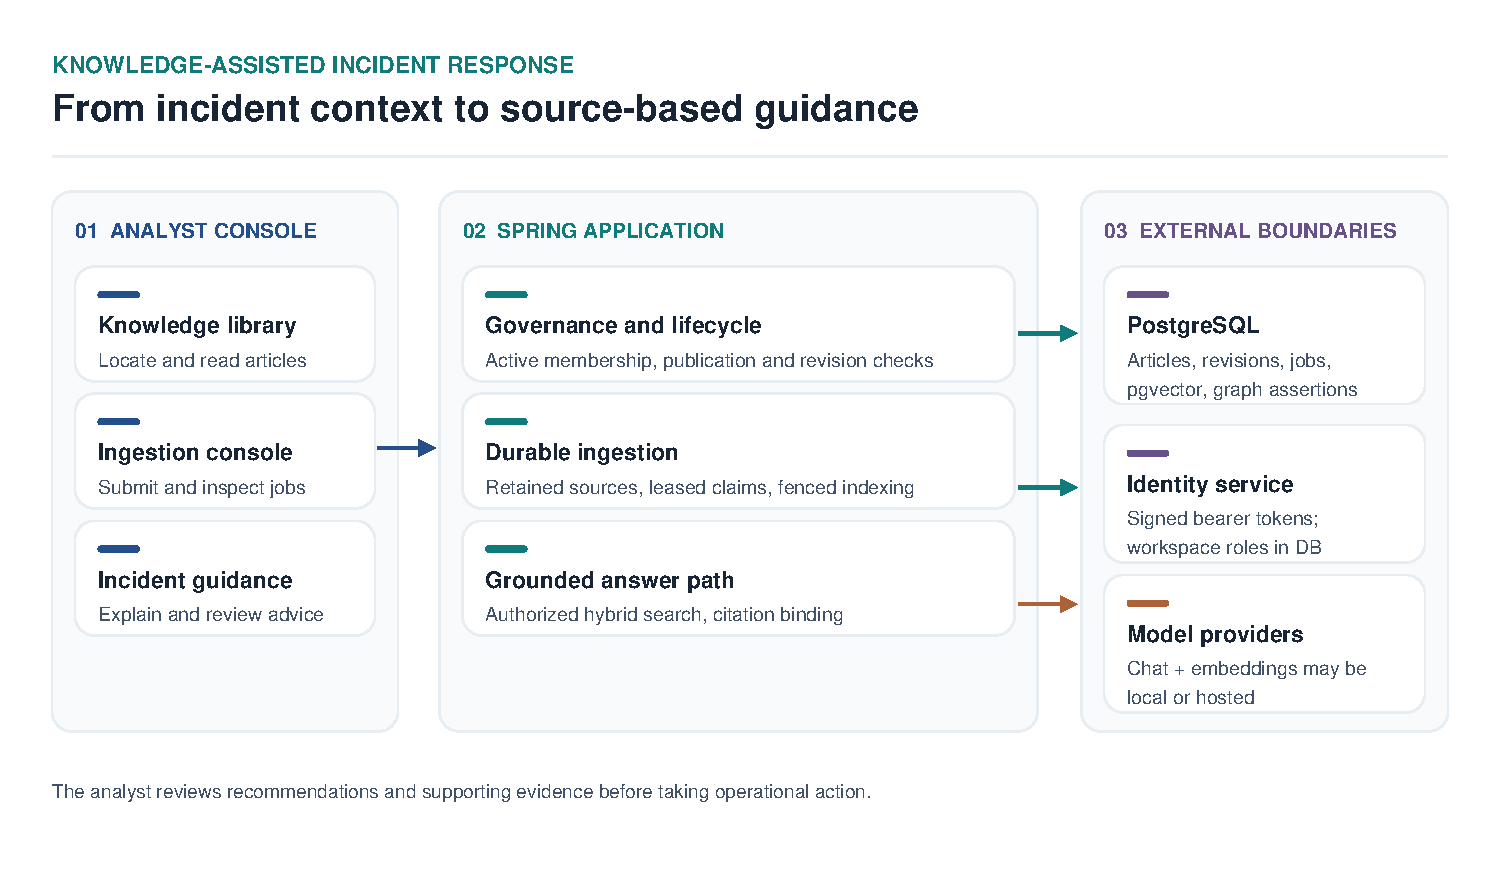
\includegraphics[width=\textwidth]{figures/architecture.pdf}
\caption{Sentinel's knowledge, application, and external-service boundaries.}
\label{fig:sentinel-architecture}
\end{figure}
\FloatBarrier

\section{Knowledge organisation and maintenance}

\subsection{Articles and curated incident playbooks}

The library organises articles by category, severity, tags, source, and update date. Article bodies contain titled sections, with related documents and indicators of compromise where applicable. These fields serve different reading tasks: a category narrows the type of knowledge, a source identifies its origin, and related documents connect an initial observation to further investigation. Severity describes the material's assigned importance; it does not diagnose the incident described by an analyst.

We include a curated collection of response playbooks to give the assistant procedural material alongside advisories and technical descriptions. Its scenarios include phishing, ransomware, account takeover, exposed credentials, application compromise, data exposure, and recovery. Each playbook follows a recognisable structure: applicability, questions to answer, first actions, evidence to preserve, containment and recovery, verification, and escalation. Decision checkpoints explain where context changes the response. For example, the phishing guidance distinguishes receiving a message from entering credentials or executing a downloaded file. We include these distinctions so that retrieved material can address the reported interaction rather than describe the threat only.

The playbooks are source-attributed editorial syntheses, identified as AI-assisted and requiring human review. Their admission checks require attribution, declared categories, consistent identifiers, and the review notice; they also exclude unverified indicators from this general guidance. Installation adds missing articles through the governed publication process and preserves existing content when it differs. A custodian must review such differences rather than lose local adaptations during a refresh. Here, approval permits reference use; operational applicability still depends on review in the receiving organisation.

\subsection{Review, publication, and reuse}

An editor can create a draft revision and submit it for review while the current approved article remains available. Administrative approval rejects self-approval and publishes the accepted revision. Rejection leaves the existing publication intact. State-version checks detect a decision based on an outdated workflow state, which matters when several custodians are maintaining the same procedure. This workflow supports knowledge improvement without making unfinished advice available to the assistant.

Supersession publishes a reviewed successor, whereas administrative rollback creates a new revision from previously published content. Rollback preserves a forward-moving revision history and uses a separate administrative publication route. Expiry removes material from present read eligibility while retaining its history. These operations make maintenance part of knowledge reuse: a response procedure can remain attributable without remaining suitable for current advice.

The publication transaction also records durable reindex work. Replacement is tied to the intended revision and governance state, so a delayed worker cannot publish search material for an obsolete state. During reindexing, an approved revision may temporarily lack searchable embeddings. We favour this gap over allowing superseded guidance to enter a new answer simply because its vectors are still stored.

We keep saved answers separate from published guidance. A conversation can support follow-up work, while knowledge custodians decide which lessons belong in a revised article. This separation prevents a generated response from acquiring publication authority merely because it has been retained. Reuse therefore depends on editorial judgement as well as the ability to search prior knowledge.

\subsection{Maintaining externally supplied knowledge}

Source connectors complement local material with vulnerability and incident information. Refreshes for NVD, CISA KEV, and SANS ISC use persisted work queues, progress records, and source checkpoints. Unchanged records retain their revision; changed source-owned records receive new revisions and evidence. Manual policy or content changes require review instead of being silently overwritten by a feed. Fetching and reindexing remain separate stages, so connector progress and search readiness answer different operational questions.

Trusted producers can publish reference material through an explicit admission route without manual review of each item. This is a decision about which producers the KMS accepts, with the corresponding maintenance responsibility assigned to its operators. Together with the curated collection and editor-managed articles, it gives the library several acquisition routes while retaining a common publication and evidence model.

\section{Recoverable ingestion of local and remote sources}

Incident knowledge also arrives as uploaded documents or material imported from a URL. Sentinel checks uploads for accepted formats and size, assigns source identities, and retains their content before exposing a queued job. URL admission checks the destination; the worker retains the first successful response before extraction. A retry consequently processes the same retained material rather than relying on an open browser session or downloading an unnoticed replacement. Optional owner-scoped request identifiers allow repeated submissions of the same request to recover its existing job.

Processing separates extraction, sanitisation, chunking, embedding, and indexing. For uploaded text, the configured chunker uses character windows of 1200 characters with an overlap of 150. Overlap retains some context across boundaries, while fixed windows keep processing predictable across document formats. The tradeoff is that a window may divide a sentence or procedure. Governed articles instead provide retained evidence passages with explicit identities. Missing source content or empty extraction produces a failed job that can be inspected and, when appropriate, retried.

A worker holds a time-limited claim with a token and processing generation. Progress updates and index replacement must match that live claim. Recovery advances the generation, preventing a delayed worker from overwriting a later retry or restoring deleted material. Repeated embedding calls remain possible when a worker loses its claim after contacting a provider; the protected operation is the replacement of searchable content. This design addresses F2 by preserving continuity of knowledge acquisition through interruptions.

An indexed upload retains its own access scope and processing history. Indexing alone does not turn it into an approved library article. The assistant can use an authorised upload as grounding, but article publication and article-level citations require their corresponding evidence identities. Keeping these routes distinct allows an analyst to consult submitted material without making it organisational guidance by accident.

\section{Machine-learning retrieval and incident guidance}

The assistant follows retrieval-augmented generation (RAG): it retrieves knowledge for the reported situation and supplies that material to a language model. We use machine learning for representation and explanation, while explicit application rules determine which knowledge is eligible and how its use can be inspected.

\subsection{Combining semantic and lexical retrieval}

Machine learning enters retrieval through embeddings: numerical representations of passages and questions produced by an embedding model. Sentinel compares the question representation with stored passage vectors using cosine distance. We use this route to address differences between the language of a report and the terminology of the library. A person may describe encrypted files without naming the relevant response category. Lexical search supplies a complementary route for terms and identifiers that appear explicitly in the question and stored text.

Both searches apply article eligibility and access conditions before limiting their candidate lists. Eligible article passages belong to the current approved, active, unexpired revision and match a retained evidence span. Upload candidates follow their durable-source access rules. Filtering at this point allows accessible material to compete for the available positions instead of first filling them with inaccessible matches. If vector retrieval fails, lexical retrieval still applies the same access conditions.

We combine the two ranked lists using reciprocal-rank fusion~\cite{cormack2009rrf}. For passage $d$, the ordering score is
\begin{equation}
 F(d)=\sum_{\ell\in\{\mathrm{vector},\mathrm{lexical}\}:d\in\ell}
 \frac{1}{60+\operatorname{rank}_{\ell}(d)}.
\end{equation}
The configured fusion constant is 60; ranks begin at one. This choice combines positions rather than treating cosine similarity and lexical relevance as directly comparable quantities. A passage found by both methods accumulates a contribution from each list. The score determines ordering, not the probability that advice is correct. The configured minimum similarity applies to vector candidates, while category and minimum-severity filters use article metadata in both searches.

\subsection{Establishing the context for an answer}

The assistant supplements hybrid retrieval with access-aware indicator lookup. This gives literal technical observations a route to matching knowledge alongside the broader semantic search. Indicator lookup uses the original question and is separate from the hybrid search's category and severity filters. Its evidence span identifies the indicator occurrence; a surrounding summary still needs to be checked against the full article. After combining candidates, the application resolves readable articles and exact evidence references before constructing model context. An optional reranker receives only authorised candidates.

Conversational rewriting can turn a follow-up question into a standalone search question using recent turns. We place this step after literal-question retrieval has established usable evidence. If that initial retrieval is empty, the assistant returns a local message directing the analyst to refine the question or browse playbooks. This conservative ordering avoids a generated answer detached from accessible knowledge, although it can also leave a context-dependent follow-up unanswered. The question may already have reached the embedding provider during retrieval; the gate controls the subsequent rewriting, reranking, and answer-generation stages.

The prompt combines the question, bounded recent conversation, and selected sources. Each article passage carries source information and a server-issued evidence token. The source-context budget limits prompt growth, at the cost of potentially truncating the final passage. We therefore treat retained grounding references as the material selected for context, rather than a record of the model's reasoning. Knowledge remains external to the generation model: revisions can change what is retrieved without retraining it.

\subsection{Turning retrieved knowledge into response guidance}

We shape the generation instructions around the decisions an incident responder faces. For suspected incidents, the model is asked to separate observations from explanations and organise supported advice around immediate actions, investigation and evidence preservation, recovery, and verification. The instructions call for an explanation of each action's purpose, expected result, and responsible actor. They limit clarification to three focused questions and prohibit assumptions about the operating system, affected platform, or responder's administrative access.

The instructions also require the model to explain operational impact before disruptive actions and to preserve evidence before cleanup. Requests for redacted observations replace requests for passwords, secret keys, verification codes, or complete sensitive logs. A conceptual question can receive a short explanation instead of a forced incident checklist. These instructions define the intended assistance; the reviewable sources and subsequent answer assessment remain necessary because a language model can misapply them.

The application supports structured answer blocks and a natural-language conversation route. Both use the same practical guidance and authorised context. The model is instructed to copy evidence tokens supplied by the server. Response processing resolves accepted tokens to retained references and removes unsupported citation tokens. Article citations and exact-passage references are then associated with the assistant message, making the advice available for later inspection.

\subsection{Useful behaviour when generation is unavailable}

A model failure need not remove access to existing guidance. When generation fails or is temporarily blocked, Sentinel first looks for an eligible playbook among the retrieved articles. It independently resolves up to three bounded sections titled \emph{First actions}, \emph{Questions to answer}, and \emph{Evidence to preserve} from that playbook's current approved revision. The section text comes from retained evidence, with a separate access check for each passage, rather than from trusting the retrieval metadata alone.

The fallback quotes these sections and labels them as existing playbook guidance, not a personalised answer. If section expansion cannot be authorised, it provides available retrieved article references for direct reading. It does not combine fragments into a locally invented response plan. This behaviour preserves a useful part of the KMS during a generation outage while making the loss of contextual adaptation visible. The same final authorisation and citation-persistence checks apply to fallback and generated responses.

\subsection{Keeping guidance attached to evidence}

An exact article citation identifies the article, revision identity and number, evidence snapshot, and passage boundaries. Retrieval checks the passage against the retained snapshot. Figure~\ref{fig:evidence-path} follows this relationship through to inspection. An article title alone would be insufficient because the displayed article could change after the answer was produced. Retaining a passage identity makes that change distinguishable from the evidence originally selected.

Before releasing an answer, the application checks that its grounding remains authorised and persists its references. The conversation route buffers generated output before sending its server-sent events, allowing this final disclosure check to occur before text reaches the browser. The tradeoff is a longer wait for the first visible answer rather than immediate provider-token display.

Evidence inspection performs another current-access check. Superseded, expired, revoked, or otherwise unavailable references return an unavailable state, while their identities can remain in the conversation record. We prioritise present disclosure rules over unrestricted replay of previously visible passages. A resolved citation establishes which material can be inspected; deciding whether that material supports the recommendation remains an analyst and evaluation task.

\begin{figure}[htbp]
\centering
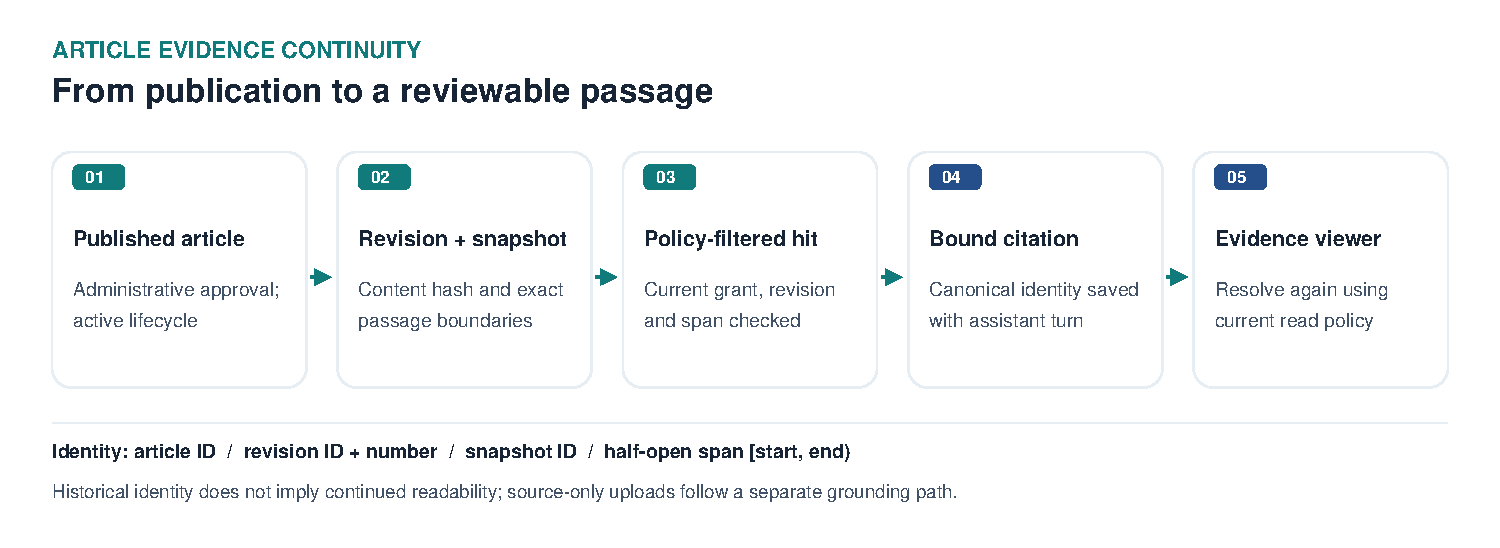
\includegraphics[width=\textwidth]{figures/evidence-path.pdf}
\caption{An editor-managed article's path from publication to access-checked evidence inspection.}
\label{fig:evidence-path}
\end{figure}
\FloatBarrier

\section{Analyst interaction and knowledge reuse}

The interface connects direct reading with conversational assistance. In the knowledge library, topic shortcuts lead to playbooks for recognisable problems such as suspicious messages, encrypted files, compromised accounts, and exposed secrets. Search, category and severity filters, and sorting support more deliberate exploration. An article opens in a reading pane with its sections, source information, and related documents. For playbooks, an action transfers a request to the assistant to help apply the selected guidance, asking about the situation and actions already taken.

The assistant accepts free-text questions and provides an optional response-plan intake. The intake asks what happened, which devices, accounts, or services are affected, and what the reporter has already done. It turns those observations into a structured question requesting priorities, evidence preservation, recovery, verification, and escalation. Unknown fields remain explicitly unknown. This design gives the retrieval and generation stages more context without forcing the reporter to classify the incident before asking for help.

Saved conversations support follow-up and handover; answers can be copied, exported, and rated for usefulness. The response separates article navigation from exact-evidence inspection. Opening a source provides broader reading, whereas the passage action opens the cited revision and span. The dialog checks that the returned identity matches the request and manages keyboard focus while open. This distinction supports both understanding the procedure and checking the specific material associated with an answer.

The ingestion view presents source submission, processing stages, job status, retry controls, and connector refresh. These controls expose the difference between adding material and having it ready for retrieval. Figures~\ref{fig:knowledge-ui}--\ref{fig:evidence-ui} illustrate selected interface states using the actual frontend with deterministic mocked authentication and application responses. Their article text, answers, passages, and counters are demonstration data, not corpus measurements, model results, or observations from an analyst study.

\begin{figure}[htbp]
\centering
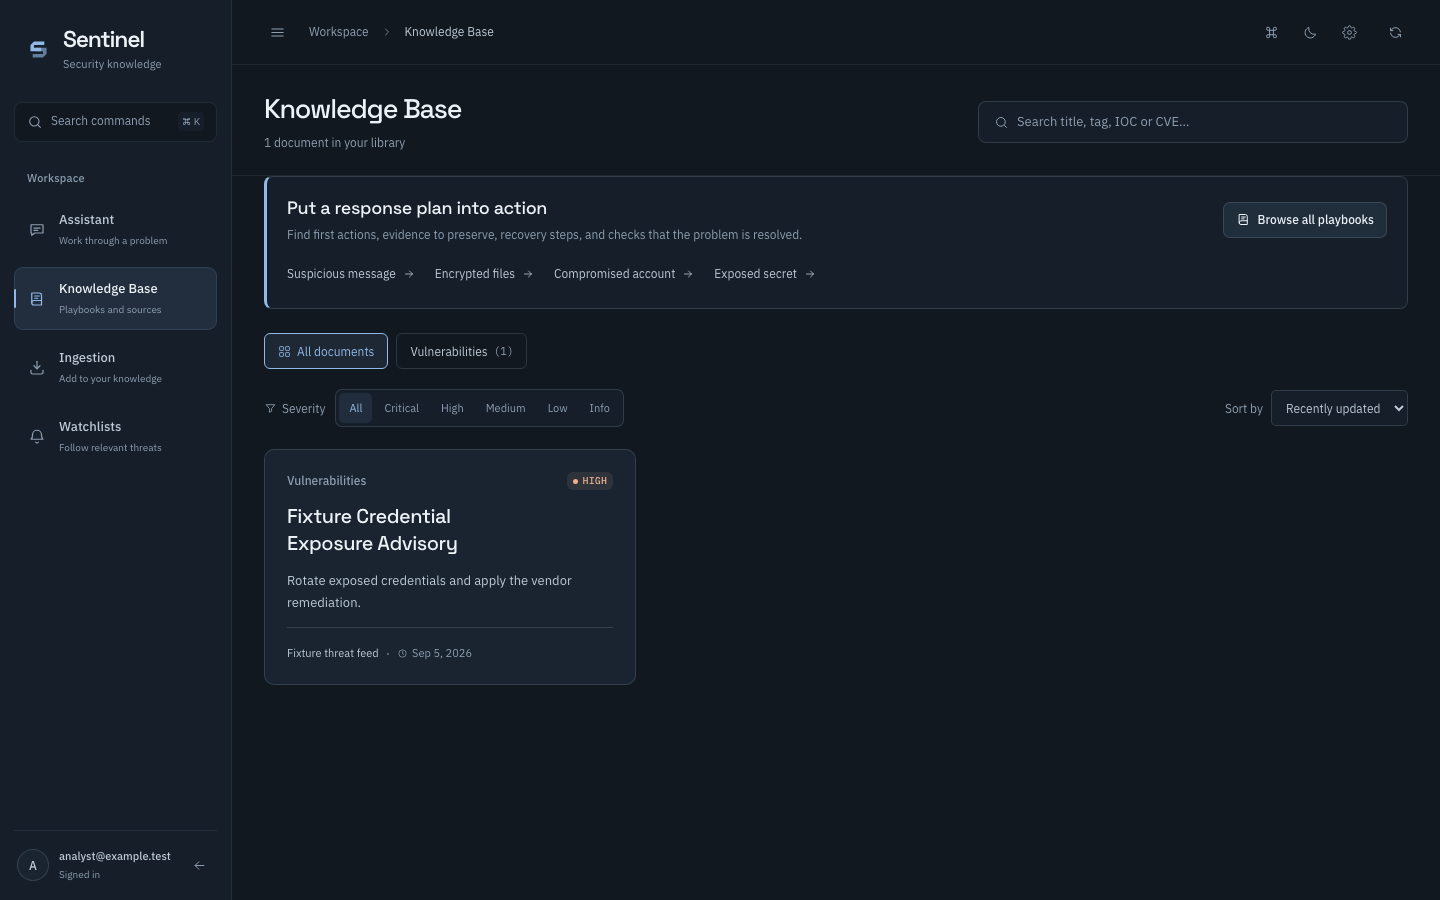
\includegraphics[width=\textwidth,trim=230bp 155bp 15bp 65bp,clip]{figures/main-knowledge-base-mocked.png}
\caption[Knowledge-library filters and playbook browsing (mocked data).]{Knowledge-library filters and problem-oriented playbook browsing (mocked data).}
\label{fig:knowledge-ui}
\end{figure}

\begin{figure}[htbp]
\centering
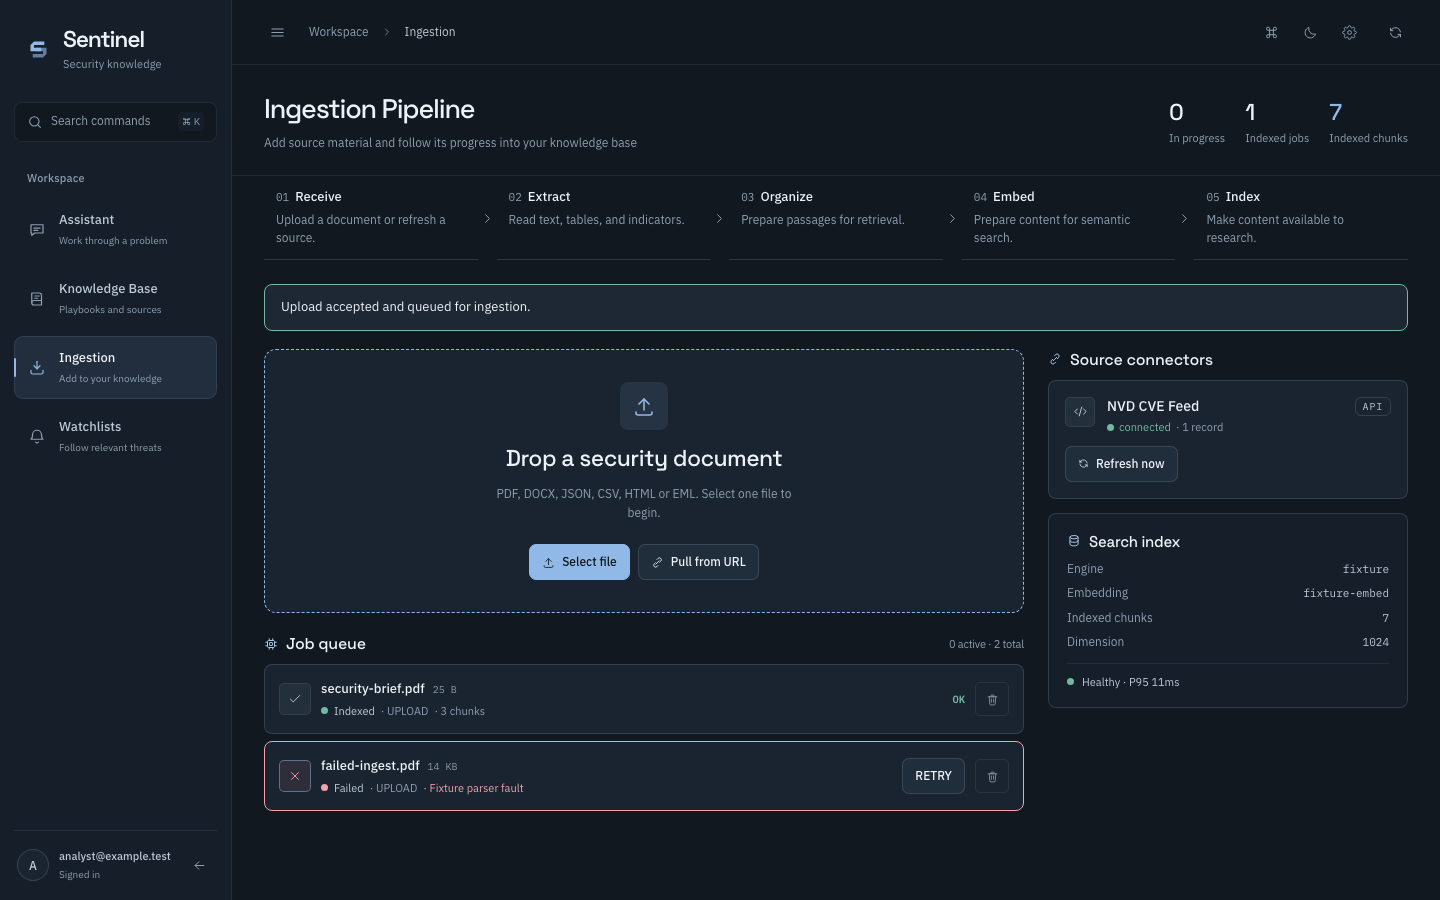
\includegraphics[width=\textwidth,trim=230bp 560bp 15bp 65bp,clip]{figures/main-ingestion-mocked.png}
\caption{Ingestion stages and source-submission acknowledgement (mocked data).}
\label{fig:ingestion-ui}
\end{figure}

\begin{figure}[htbp]
\centering
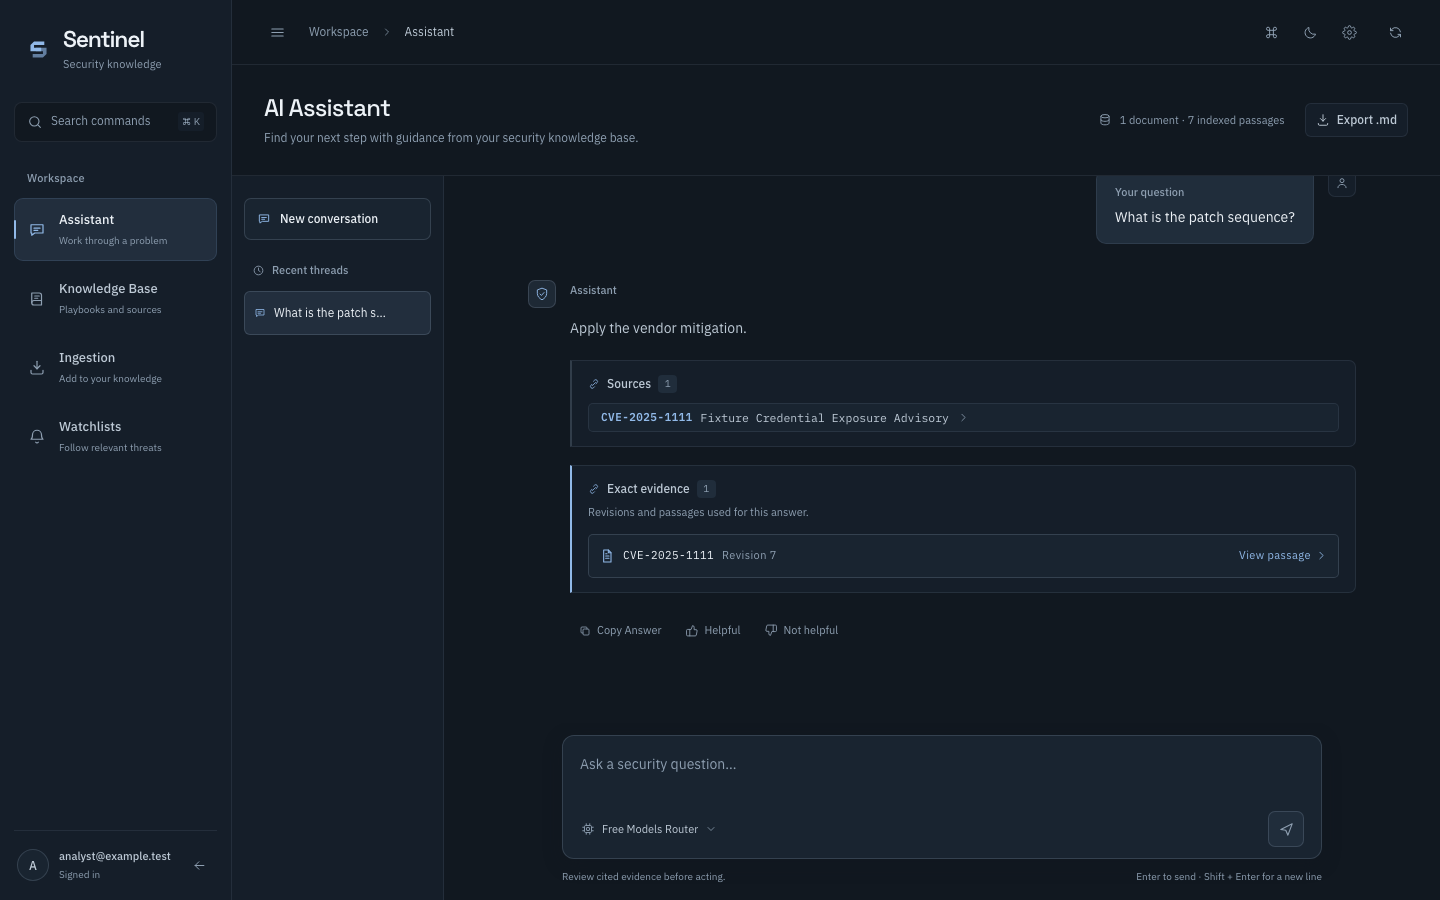
\includegraphics[width=\textwidth,trim=440bp 220bp 60bp 175bp,clip]{figures/main-cited-answer-mocked.png}
\caption{Assistant answer with article and exact-passage actions (mocked data).}
\label{fig:assistant-ui}
\end{figure}

\begin{figure}[htbp]
\centering
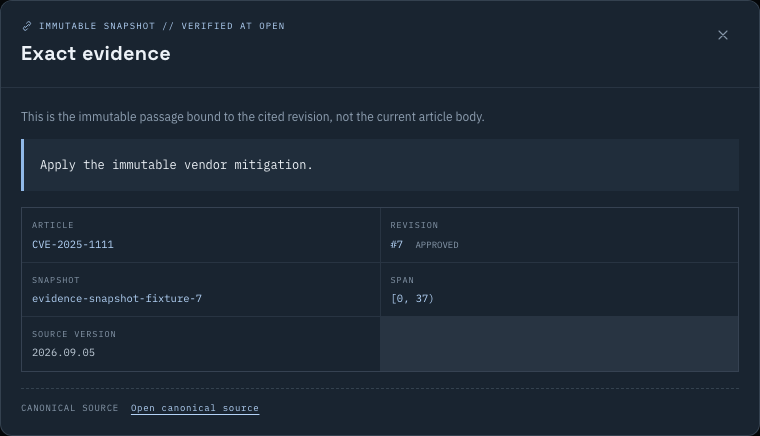
\includegraphics[width=0.85\textwidth]{figures/main-evidence-detail-mocked.png}
\caption{Evidence dialog identifying the cited revision and passage (mocked data).}
\label{fig:evidence-ui}
\end{figure}
\FloatBarrier

\section{Confidentiality and operational choices}

Access policy supports knowledge sharing at different levels. Public articles require authentication; internal material requires workspace membership; confidential and restricted material require editor and administrator authority respectively. Active database memberships determine those roles. Missing or inconsistent governance results in denial. These controls apply to direct reading, retrieval, and evidence disclosure, so a conversational request does not provide an alternative route around the library's restrictions.

Retrieved content is treated as untrusted data. Sanitisation targets recognisable injection patterns before uploaded text is indexed and before source text enters a prompt. The prompt distinguishes source material from instructions. These defences reduce exposure to known patterns but require adversarial evaluation, particularly when unfamiliar documents are admitted. The separation of source permissions from text and metadata remains necessary even when sanitisation leaves a passage apparently harmless.

For N2, revision and workflow histories describe knowledge changes, while job records explain processing progress. Redacted audit events record consequential operations and outcomes. Successful transactional changes produce their success events after the transaction completes. Audit persistence is best-effort: an audit failure is logged without replacing the original operation's result. This favours service continuity but leaves a completeness limitation that operators must consider when investigating an incident involving the KMS itself.

For N3, chat and embedding services can use hosted providers or local models through Ollama. Database and identity hosting are configured separately. Choosing local inference therefore addresses model processing, while the complete disclosure boundary also depends on where knowledge and identity services run. Hosted embedding requests transmit passage or question text; hosted answer requests transmit the question, selected context, and recent conversation. Access eligibility within the KMS and permission to send material to a provider are separate deployment considerations.

The vector store expects 1024-dimensional embeddings. Replacing the embedding model requires reindexing; a different dimensionality also requires a storage change. Reproducibility and confidentiality depend on these deployment choices, not only on the chat model.

\section{Chapter synthesis}

Sentinel connects knowledge acquisition, retrieval and response guidance. Playbooks supply procedures; embeddings and lexical search locate passages; generation relates them to the incident. Direct reading and fallback preserve access when generation fails. Chapter~\ref{ch:evaluation} examines this design against its requirements, distinguishing technical operation from the quality and usefulness of the assistance.

\chapter{Evaluation and Results}\label{ch:evaluation}

\section{Evaluation approach}

The evaluation examines whether Sentinel connects maintained knowledge to useful support for incident-response decisions. Following Chapter~\ref{ch:introduction}, we interpret optimisation as reducing the time and effort needed to locate applicable knowledge while supporting correct, well-founded decisions. A faster answer is therefore not sufficient: the retrieved material must address the situation, the explanation must preserve its meaning, and the analyst must be able to assess its applicability.

We completed model comparisons and human evaluation as part of the research, alongside engineering verification. We distinguish these activities by their object of assessment. Software checks examine specified application behaviour. Live provider calls establish compatibility with particular services. Comparative model results concern retrieval and generated responses, while human evaluation connects the assistance to its use and interpretation. These perspectives contribute to the same research objective without sharing a common unit of observation.

We use retrieval quality, response quality, task efficiency, and usability as analytical dimensions. Access restrictions and provenance apply across them: useful knowledge must be available to the intended reader, and the basis of advice must remain inspectable. The following definitions establish the meaning of these dimensions before the technical results and their relationship to RQ1--RQ3 are discussed.

% EDITORIAL: The controlled model comparison and human evaluation were completed
% personally by the researcher. Their numerical records are awaiting transfer.
% Integrate their actual methods and findings at the marked locations below;
% absence of transferred records does not mean absence of measurement or study.

\section{Evaluation dimensions}

\subsection{Retrieval quality}

Retrieval quality concerns whether the returned knowledge helps answer the incident question. Topical similarity is only one part of relevance. A passage about account compromise may describe the correct threat but omit the recovery procedure or the conditions governing its use. Article-level relevance identifies a useful document; passage-level relevance asks whether the selected text contains the information needed for the decision. We distinguish these units because an appropriate article can still yield an incomplete context for generation.

Precision describes the proportion of retrieved items judged relevant, whereas recall describes the proportion of the relevant set recovered. A ranking cutoff limits the results considered. Mean reciprocal rank summarises the position of the first relevant result, and normalised discounted cumulative gain assesses the ordering of relevant material against an ideal ranking. These measures distinguish finding some useful evidence from recovering the evidence needed to address the whole question.

The reference set also depends on access and temporal scope. Material outside the requesting identity's permissions is not an eligible target, and superseded guidance may be relevant to a historical question without being appropriate for current advice. Questions with no relevant accessible evidence form a distinct category; recall has no meaningful denominator for an empty reference set. Returning unrelated material in that situation is different from failing to retrieve an available answer.

\subsection{Response quality and traceability}

Response quality concerns how the assistant uses knowledge, not merely whether it produces fluent text. RAGAs distinguishes retrieval of useful context, faithful use of that context, and generation quality. ARES similarly separates context relevance, answer faithfulness, and answer relevance~\cite{ref039,ref040}. We adopt this separation as an analytical basis for examining guidance without treating any one dimension as a complete measure of correctness.

Relevance concerns whether the response addresses the question. Faithfulness concerns whether its claims are supported by the supplied material. Correctness additionally concerns whether the advice is accurate and applicable to the stated situation. Completeness concerns the information necessary to make the decision, including important qualifications and dependencies. For example, quoting a recovery action faithfully does not make the advice complete if the source also requires evidence preservation before that action. A response can thus be well grounded and still omit something consequential.

Traceability makes the supporting material available for examination. Citation resolution establishes that a reference identifies an inspectable source and passage. Citation support concerns whether that passage justifies the associated statement; citation coverage concerns how much of the evidence-requiring advice has adequate support. Sentinel's retained passage identities address the first problem, while the meaning of a claim--passage relationship remains a quality question.

Uncertainty is part of this assessment. A useful response distinguishes observed facts from hypotheses and recognises insufficient evidence. Appropriate abstention avoids unsupported guidance; unnecessary abstention withholds assistance despite adequate evidence. Likewise, error severity matters: an imprecise explanation and a recommendation that risks destroying incident evidence have different consequences. These distinctions connect language quality to the decisions the KMS is intended to support.

\subsection{Task efficiency and usability}

Task efficiency concerns the effort needed to reach a justified response decision. It includes finding sources, reading them, checking the explanation, and deciding what applies. Model latency measures only part of this work. Time to first visible output and time to a complete answer also describe different experiences, particularly because Sentinel checks the grounding before releasing a generated response.

We interpret efficiency together with decision quality. Rapid acceptance of unsupported advice is not an improvement in incident response. Conversely, additional time spent checking a critical passage may support a better decision. The relevant comparison is therefore between task outcomes and the effort associated with them, rather than between response times alone.

Usability concerns how readily people can navigate the knowledge, express their question, understand the response, and inspect its basis. Perceived usefulness and confidence describe the experience of using the system; they do not establish correctness. The ability to recognise an unavailable source or challenge a recommendation is also relevant to usability because successful interaction includes knowing when further investigation is necessary.

\section{Engineering results}

Software verification on 29 September 2026 covered report validation, backend behaviour, frontend components, scripted browser interactions, and production frontend packaging. Table~\ref{tab:executed-checks} presents the observed results as separate layers. The backend total was obtained from 88 test reports, with no failures, errors, or skipped tests. Selected backend checks used isolated PostgreSQL instances alongside mocked dependencies.

\begin{table}[htbp]
\centering\small
\caption{Engineering checks completed on 29 September 2026.}
\label{tab:executed-checks}
\begin{tabularx}{\textwidth}{@{}>{\raggedright\arraybackslash}p{0.24\textwidth}>{\raggedright\arraybackslash}p{0.23\textwidth}>{\raggedright\arraybackslash}X@{}}
\toprule
\rowcolor{TableNavy}
\color{white}\bfseries Check & \color{white}\bfseries Observed result & \color{white}\bfseries Scope \\
\midrule
\rowcolor{TableStripe}
Report validator & 12 tests passed & Acceptance and rejection of synthetic evaluation and test reports. \\
Backend tests & 408 tests passed & Application rules and selected isolated database interactions. \\
\rowcolor{TableStripe}
Frontend unit tests & 91 tests passed & Component behaviour in a simulated browser document. \\
Chromium tests & 17 tests passed & Scripted navigation and intercepted application-response contracts. \\
\rowcolor{TableStripe}
Production frontend build & Succeeded; 133 modules transformed & Packaging of the interface for production use. \\
\bottomrule
\end{tabularx}
\end{table}

The report validator checks the consistency and acceptability of declared results, including invalid metrics and misleading pass declarations. Its synthetic inputs exercise reporting logic rather than retrieval effectiveness. The application suites address a different object: whether selected operations behave as expected under the tested conditions. The production build completed with a non-fatal bundle-size warning, establishing successful packaging rather than a deployed service.

The interface illustrations in Chapter~\ref{ch:system} use deterministic mocked authentication and application responses; their displayed answers, passages, and counters are demonstration data, not human-evaluation observations. The browser checks support the operation of those interface interactions. Together, the engineering results establish a functioning basis for knowledge access and evidence inspection, but their test counts are neither incident samples nor measures of decision quality.

\section{Live provider compatibility}

Live compatibility observations on 6 September 2026 examined embedding services through OpenRouter using a requested dimension of 1024, matching Sentinel's vector storage. The endpoints \nolinkurl{nvidia/llama-nemotron-embed-vl-1b-v2:free} and \nolinkurl{liquid/lfm-2.5-embedding-350m:free} returned 1024-dimensional vectors, each with a reported cost of zero. In contrast, \nolinkurl{nvidia/nemotron-3-embed-1b:free} returned HTTP~400 with a requirement for 2048 dimensions.

The same dated record describes a completed live chat request, a batch of two 1024-dimensional embeddings, and a synthetic vector inserted into PostgreSQL with pgvector, queried using cosine distance, and subsequently rolled back. These observations demonstrate provider connectivity and the vector write/query path. They do not constitute a model-quality comparison or a complete authenticated ingestion-to-answer trial. The available account does not include repetition counts or raw response logs from which reliability or latency distributions could be estimated.

The dimensionality difference has a direct engineering consequence. A model requiring 2048 dimensions cannot populate the existing 1024-dimensional representation without a storage change. Matching dimensions, however, does not make different models' representations interchangeable: replacing the embedding model also requires reindexing the knowledge with the selected representation. We therefore interpret successful responses as compatibility observations for the named services on the recorded date. Reported zero cost describes those responses, not a standing guarantee of availability, pricing, or the absence of infrastructure costs.

\section{Model comparisons and human evaluation}

\subsection{Interpreting model comparisons}

A model comparison describes performance under particular knowledge and configuration conditions. The embedding model affects which material is retrieved, while the generation model affects how the supplied material is expressed. Corpus coverage, passage boundaries, context limits, and access permissions also shape the available evidence. A difference between complete configurations therefore cannot automatically be attributed to one model or to retrieval alone.

We distinguish retrieval outcomes from answer outcomes when interpreting comparative performance. An improved ranking can make supporting knowledge easier to find without ensuring that the answer uses it correctly. Similarly, a convincing answer may rely on general model knowledge rather than the maintained collection. The relationship between the question, retrieved passages, response, and quality judgement is consequently more informative than a single aggregate score. Failed requests also belong to the interpretation of a configuration's practical usefulness, alongside the quality of its successful responses.

% EDITORIAL -- completed controlled comparison, method integration:
% Insert the actual study dates, evaluated system configuration, model/provider
% identifiers, corpus composition and size with units, case-selection process,
% comparison conditions, repetitions, prompts, retrieval settings, generation
% settings, access context, and scoring method from the original records.
% Describe only conditions actually used; do not infer search-only, no-RAG, RAG,
% paired allocation, held-out splits, reviewer independence, or randomisation.
% EDITORIAL -- completed controlled comparison, results integration:
% Incorporate original per-case rankings, responses, relevance judgements,
% quality labels, timing units and measurement boundaries, failed attempts,
% usage/cost observations, and their denominators, or labelled aggregate records
% stating those details. Add result tables only when values and provenance are
% available. Reconcile any contract-example metrics with the primary records
% before treating them as observations. Calculate uncertainty only when the
% actual sampling and repetition structure support the chosen analysis.

\subsection{Interpreting human evaluation}

Human evaluation connects the system's outputs to how people understand and use knowledge. We distinguish assessments of an answer from assessments of interaction with the KMS. Judging the clarity of a displayed recommendation concerns the response; locating its source, checking applicability, and reaching a decision concern a broader task. This distinction determines how far an observation can support a claim about incident-response work.

Quantitative outcomes and qualitative feedback also answer different questions. A task-time observation describes elapsed work under defined conditions, while a comment about saving time expresses perceived value. Feedback can explain difficulties with terminology, source navigation, or the amount of detail without establishing their frequency across other users. Evidence consultation is similarly interpretable only in context: opening a passage demonstrates access to it, not necessarily understanding or appropriate reliance.

% EDITORIAL -- completed human evaluation, method integration:
% Insert documented dates, participant count and relevant experience in
% anonymised form, recruitment, materials, tasks or review activity, conditions
% actually encountered, task order/allocation if recorded, and instruments with
% their exact scales and scoring. Distinguish answer review from interactive
% task performance. Describe consent, approval and data handling only from
% supporting records; do not infer approval, randomisation or blinding.
% EDITORIAL -- completed human evaluation, results integration:
% Incorporate recorded task outcomes and times, questionnaire item responses or
% labelled aggregates, and attributable anonymised qualitative evidence, as
% available. Preserve participants, task attempts and model outputs as distinct
% denominators; identify missing responses, exclusions and failures. State the
% qualitative analysis actually performed. Do not infer a usability instrument,
% participant benefit, significance, themes or quotations from demonstrations.

\section{Requirement validation and discussion}

Table~\ref{tab:evaluation-status} relates the requirements in Chapter~\ref{ch:system} to the scope of the documented technical evidence. Functional requirements connect knowledge maintenance to guidance; the non-functional requirements concern the conditions under which that guidance remains usable and reviewable. This relationship prevents successful software checks from being treated as acceptance of every research objective.

\begin{table}[htbp]
\centering\small
\caption{Requirements and the scope of the documented technical evidence.}
\label{tab:evaluation-status}
\begin{tabularx}{\textwidth}{@{}>{\raggedright\arraybackslash}p{0.23\textwidth}>{\raggedright\arraybackslash}p{0.30\textwidth}>{\raggedright\arraybackslash}X@{}}
\toprule
\rowcolor{TableNavy}
\color{white}\bfseries Requirement & \color{white}\bfseries Assessment focus & \color{white}\bfseries Evidence and interpretation \\
\midrule
\rowcolor{TableStripe}
F1 Governed knowledge & Currency and controlled publication. & Lifecycle checks support the maintenance mechanisms, not the suitability of every article. \\
F2 Recoverable ingestion & Continuity from retained source to index. & Backend recovery checks include isolated database interactions. \\
\rowcolor{TableStripe}
F3 Contextual retrieval & Relevant, accessible knowledge. & Search behaviour is technically checked; relevance belongs to comparative quality assessment. \\
F4 Traceable incident guidance & Advice linked to inspectable evidence. & Citation resolution and viewing are checked separately from semantic support. \\
\rowcolor{TableStripe}
N1 Access and disclosure safety & Permissions across retrieval and disclosure. & Selected authorisation checks support defined boundaries, not a general security guarantee. \\
N2 Reviewable operations & Examination of changes and failures. & Retained histories support inspection; best-effort audit persistence limits completeness. \\
\rowcolor{TableStripe}
N3 Deployment flexibility & Separation of hosting and model choices. & Successful packaging and dated provider compatibility observations. \\
\bottomrule
\end{tabularx}
\end{table}

For RQ1, the design and requirements analysis identify procedures, applicability conditions, and the rationale for decisions as reusable knowledge, accompanied by provenance and maintenance responsibility. The lifecycle mechanisms make that organisation actionable through review, publication, and revision. RQ2 connects this maintained collection to guidance through semantic and lexical retrieval, source-conditioned generation, and exact-passage inspection. The technical evidence supports the operation of selected parts of this chain; the quality dimensions distinguish relevant retrieval from a justified recommendation.

RQ3 brings those dimensions together with task efficiency and usability. Its interpretation depends on the model and human findings rather than on a combined software-test total. The principal issue is whether reduced effort accompanies sounder use of knowledge, including appropriate recognition of uncertainty and access limits.

\subsection{Limitations of interpretation}

The engineering suites cover selected inputs and environments. They establish application behaviour under those conditions, rather than whether a security recommendation is appropriate or a cited source is correct.

The compatibility observations and engineering checks concern different dates and activities. Neither identifies the configuration used in the model comparison or human evaluation. Provider selection, knowledge revisions and permissions can change the evidence available to a question; comparative findings therefore concern the documented configuration.

Human findings likewise concern the documented participants, tasks and setting. Experience, familiarity with the interface and repeated exposure to cases can affect performance. Their relevance depends on the actual study conditions, alongside the distinction between technical operation and its contribution to response decisions.

% EDITORIAL -- final synthesis: After integrating the completed empirical work,
% connect its actual findings to RQ1--RQ3 and the requirement matrix. State the
% supported magnitude and scope of any retrieval, response-quality, efficiency
% or usability benefit, including unfavourable findings. Revise limitations to
% reflect the documented study design rather than an assumed future protocol.

\chapter{Conclusion}\label{ch:conclusion}

This dissertation examined how a knowledge-management system can use machine learning to support cybersecurity incident-response decisions. We developed Sentinel to connect maintained articles and response playbooks with contextual retrieval and source-based explanations. The starting point was a practical knowledge-management problem: an analyst needs the conditions and rationale behind a procedure, not only the document containing it. We therefore treated capture, maintenance and reuse as parts of the same task, with the analyst retaining responsibility for action. Optimisation means reducing the effort needed to reach a correct, well-supported decision, rather than simply producing an answer more quickly.

\section{Answers to the research questions}
For RQ1, our design answer is to retain procedures, threat-related material and incident lessons with the context needed to judge their applicability. A playbook needs conditions, responsibilities and verification steps; an incident lesson needs the observations and reasoning behind an earlier decision. In Sentinel, classified articles, source attribution, revisions, publication review and expiry provide a way to maintain that knowledge. Retained uploads and recoverable processing extend acquisition without making every submitted document approved organisational guidance. Saved conversations likewise remain separate from published knowledge, so reuse includes an editorial decision rather than automatic promotion of generated text.

RQ2 connects this knowledge to the analyst's question. We combine embeddings from pretrained models with lexical retrieval and indicator lookup, allowing semantic similarity and explicit technical terms to contribute to passage selection. The language model receives authorised source material and instructions to distinguish reported observations from possible explanations, relate actions to their purpose and preserve uncertainty. Article and passage references connect the response to inspectable knowledge. Machine learning supports representation and explanation; it does not determine publication authority or execute remediation. When generation is unavailable, eligible playbook excerpts or direct article references provide an alternative route to the existing guidance. This design uses pretrained models at inference time rather than training a new incident-response model.

For RQ3, the documented engineering checks establish selected processing, access and interface behaviours under their test conditions. The live provider calls reported in Chapter~\ref{ch:evaluation} distinguish accepted requests from an embedding configuration rejected at the requested dimension. These observations concern technical operation; they do not quantify retrieval relevance, answer correctness or analyst efficiency. We distinguish those outcomes from usability and interpret task time alongside the quality of the resulting decision. A resolved citation, a completed model request and a correct incident-response decision answer different evaluation questions.
% RQ3 quantitative synthesis: integrate the transferred records of the completed controlled model comparisons and human evaluation here, consistently with Chapter 4. Retain actual conditions, case and participant denominators, failures, scoring rules and uncertainty; report only outcomes present in those records.
% Reserve the effectiveness answer and any comparative claim about retrieval, response quality, task efficiency or usability until that synthesis is available. Missing transferred records do not mean the evaluations were not conducted. Do not infer model rankings, participant findings or effect sizes from technical checks, compatibility calls or illustrative examples.

\section{Contributions and limits}
The principal contribution is the connection between maintained knowledge and an incident question. An analyst can describe suspicious activity, consult retrieved guidance, inspect its supporting passage and return to the broader procedure. Knowledge custodians can revise that procedure without retraining the language model. By bringing these activities together, we give knowledge management a direct role in response assistance, while keeping responsibility for the underlying content visible. The contribution is an integration of established methods around incident-response work, rather than a new retrieval algorithm.

The design also makes the distinction between source access and advice review concrete. The reading interface exposes both the article and the particular passage associated with an answer. This supports checking a recommendation against its context, but an exact reference does not prove that every generated statement follows from the passage. Nor does a relevant source establish that its procedure applies to the affected environment. The analyst still needs to assess prerequisites, operational consequences and uncertainty before acting.

Several choices constrain the context available for that assessment. Fixed passage boundaries and a limited generation context can separate an instruction from a qualification. Literal-question retrieval can miss a follow-up that needs conversational context. Publication and indexing occur separately, so an approved revision may temporarily be unavailable to semantic search. Current access rules can also make a previously cited passage unavailable. We accept these last two restrictions to avoid reusing obsolete or no longer authorised material. The graph assertion store records evidence-linked relationships; the assistant does not traverse it to retrieve knowledge.

Deployment introduces a separate set of boundaries. Local chat or embedding inference does not establish that storage and identity services are local, and an external model service receives the material sent to it. Access within the KMS and permission to disclose knowledge to a provider are therefore distinct decisions. Operational records also remain best-effort rather than a guarantee of complete event capture. These limits affect how the system can be used and investigated; they are not measures of model quality or substitutes for assessing decisions in their operational setting.

\section{Further development}
We see useful extensions in preserving procedural context during passage construction and improving follow-up retrieval without bypassing evidence eligibility. Structure-aware passages could keep prerequisites with the actions they qualify. A revised conversational search strategy could use earlier observations while retaining a clear response when accessible evidence is insufficient. Both extensions address specific ways in which relevant knowledge can be lost between a source and an answer.

A more direct route from a reviewed incident lesson to a proposed article revision could also make experience easier to retain, while leaving publication with the responsible custodians. The aim would be to preserve why a decision was made and when it applies, not to treat a saved conversation as automatically learned organisational knowledge. Linking an exception to the procedure it changes would help the next responder identify the relevant qualification.

Sentinel provides an implemented approach to the architectural part of the principal research question: maintained knowledge supplies the content, machine learning supports its retrieval and explanation, and analysts decide how to use it. The criterion for optimisation remains the quality of that decision together with the effort required to reach it. This keeps incident-response knowledge reuse, rather than the fluency of generated text, at the centre of the contribution.
% Reconcile the closing synthesis with the transferred RQ3 results after their integration, retaining this distinction between implemented capability and measured effectiveness.

\appendix
\chapter{Knowledge lifecycle and incident scenario}\label{app:implementation}

This appendix develops the knowledge-lifecycle and incident-response examples introduced in Chapter~\ref{ch:system}. We use constructed examples to explain how the design connects knowledge maintenance with an analyst's decisions. They are illustrations, not observed incidents, participant task records or model outputs.

\section{A knowledge item through capture and reuse}
Consider a playbook for suspected account compromise. Its useful content includes the circumstances in which it applies, questions that distinguish possible explanations, evidence to preserve, response options and recovery checks. Responsibility for consequential actions belongs in that context: an analyst may be able to investigate a report without having authority to change an account. A reusable playbook therefore needs to describe both the procedure and the conditions governing its use.

Table~\ref{tab:scenario-checkpoints} follows this item through the design. The requirement identifiers refer to Table~\ref{tab:system-requirements}. The stages describe the implemented lifecycle, while the particular playbook and sequence form an illustrative example.

\begin{longtable}{@{}>{\raggedright\arraybackslash}p{0.18\textwidth}>{\raggedright\arraybackslash}p{0.39\textwidth}>{\raggedright\arraybackslash}p{0.35\textwidth}@{}}
\caption{Knowledge-lifecycle stages illustrated through a response playbook.}\label{tab:scenario-checkpoints}\\
\toprule
Stage and requirements & KMS behaviour & Significance for knowledge reuse \\
\midrule
\endfirsthead
\toprule
Stage and requirements & KMS behaviour & Significance for knowledge reuse \\
\midrule
\endhead
Capture (F1, F2) & An editorial contribution starts a draft revision. An uploaded source retains its content and processing state before indexing. & Processing an upload does not itself grant the material the status of approved organisational guidance. \\
Review and publication (F1) & An editor submits a revision; a different authorised administrator can approve it. Rejection leaves the existing publication intact. & Unfinished changes remain separate from the procedure currently available for reference. \\
Search readiness (F2, F3) & Publication records revision-specific indexing work. Replacement checks prevent an obsolete worker from restoring older searchable content. & Publication and semantic-search availability are distinct states; delayed processing does not justify reusing a superseded revision. \\
Retrieval (F3, N1) & Semantic and lexical search select eligible passages; indicator lookup adds another access-aware route to relevant articles. & The analyst's permitted knowledge, rather than every stored document, supplies candidate evidence. \\
Guidance (F4) & Selected passages provide context for the answer. Evidence references connect accepted citations to retained material. & An explanation can be examined alongside the knowledge used to construct its context. \\
Inspection (F4, N1) & Opening an evidence passage checks its identity and current eligibility again. & Earlier access does not confer a permanent right to retrieve the passage. \\
Revision or expiry (F1, N2) & A reviewed successor can replace the procedure; expiry removes current reading eligibility while preserving its history. & Knowledge can remain attributable after it ceases to be suitable for new operational guidance. \\
\bottomrule
\end{longtable}

The review stage in this example describes editor-managed knowledge. Trusted source producers have a separate admission route, so publication does not always mean that an administrator has manually reviewed an item. The distinction matters when interpreting provenance: source attribution identifies the origin, whereas editorial approval records a particular publication decision.

An answer's evidence reference identifies an article, its revision, a retained snapshot and the boundaries of a passage. These elements distinguish the text associated with an earlier answer from a subsequently revised article. They do not explain the model's internal reasoning or certify that a recommendation follows from the text. In the lifecycle, traceability provides something concrete to inspect; judgement about support and applicability remains separate.

\section{Illustrative incident: suspected credential disclosure}
We use the following constructed report to connect that lifecycle to an incident question:
\begin{quote}
I followed a link in a message and entered my work password. I do not know whether anything else changed.
\end{quote}
The report establishes what the person says they did. It does not establish whether the account was subsequently accessed, which service was involved or whether the responder has administrative authority. We leave these details unspecified rather than inventing them to complete the scenario.

\subsection{Knowledge needed for the decision}
In this example, a phishing playbook distinguishes receiving a message from submitting credentials or opening an executable file. Account-recovery guidance describes the applicable procedure, while a local responsibility statement identifies who can authorise and perform account changes. An earlier incident lesson could explain a relevant exception, but only if its circumstances still apply. The documents serve different purposes: a general threat description cannot replace the local authority or recovery procedure.

The assistant can use accessible passages from this material to organise an explanation. The example does not assume that all of these sources exist in every deployment. If a necessary local procedure is absent, the missing context remains a limitation on the advice rather than an invitation to invent an organisational policy.

\subsection{Interaction and decision points}
\begin{enumerate}
\item \textbf{Establish the observations.} The analyst records the credential submission as reported and keeps account compromise as a hypothesis. Focused clarification can concern the affected service, whether a file was opened and which steps have already been taken. Passwords and verification codes are not needed for this description.
\item \textbf{Locate applicable knowledge.} The incident description supplies the retrieval question. Semantic matching can connect everyday wording with a playbook, while explicit terms can support lexical matching. Access and publication rules determine which passages are eligible, independently of how strongly they match the topic.
\item \textbf{Interpret the guidance.} The explanation distinguishes evidence-preservation and investigation steps from changes that require operational authority. Any proposed action needs its source-supported purpose and conditions. A recommendation to involve the responsible account team remains advice; the KMS does not perform the account change.
\item \textbf{Inspect the basis for action.} The analyst opens the cited passage and, where needed, the wider procedure. This allows examination of prerequisites, qualifications and responsibility that a short explanation might omit. The decision depends on that applicability check, not on the presence of a citation marker alone.
\item \textbf{Retain the lesson.} A saved conversation can support handover. If the case reveals an incomplete procedure, a custodian can propose a revision through the publication workflow. Retaining the conversation does not automatically change the playbook or train the model.
\end{enumerate}

\subsection{Changes that alter the interaction}
If the first retrieval finds no usable evidence, the assistant directs the analyst to refine the question or browse available playbooks. This differs from a generation outage after relevant material has been found. In the latter situation, an eligible playbook can supply bounded excerpts labelled as existing guidance, or the assistant can provide article references for direct reading. The excerpts do not become a personalised response merely because they appear in the conversation.

A later permission change or expiry can also affect the scenario. A retained citation still identifies the material associated with the earlier answer, but opening it can return an unavailable state under current policy. This makes the distinction between historical reference and present disclosure visible to the analyst. It does not silently replace the cited passage with a different revision.

\chapter{Requirements context and evaluation records}\label{app:instruments}

\section{Requirements-gathering context}
During requirements gathering, we conducted semi-structured interviews with a research specialist to identify use cases, user roles and requirements, following the literature review. This qualitative input supported the definition of the design problem described in Chapter~\ref{ch:introduction}. Its role was requirements elicitation, distinct from evaluating the effects of the developed system on incident-response tasks. The constructed scenario in Appendix~\ref{app:implementation} is not a reconstruction of an interview or a participant's task record.

The following reporting layouts serve a different purpose again: they illustrate how model and human-evaluation records can retain the distinctions used in Chapter~\ref{ch:evaluation}. They are optional organisational aids, not reproductions of administered instruments, validated questionnaires or evidence that every listed field was collected. They contain no participant responses or measured results.
% Integrate the transferred records of the completed controlled comparisons and human evaluation without treating these illustrative layouts as the administered protocol. Retain original condition names, instruments, item wording, scoring rules and recorded denominators. Do not reconstruct interview details or participant observations from the layouts.

\section{Units of observation}
A retrieved passage, a generated answer and an analyst's final decision are related but distinct observations. A relevant document may yield an incomplete passage; a supported explanation may still be unsuitable for the affected environment. Table~\ref{tab:evaluation-record-units} separates these levels so that a result retains the meaning of what was actually assessed.

\begin{longtable}{@{}>{\raggedright\arraybackslash}p{0.18\textwidth}>{\raggedright\arraybackslash}p{0.36\textwidth}>{\raggedright\arraybackslash}p{0.38\textwidth}@{}}
\caption{Evaluation units and their interpretation.}\label{tab:evaluation-record-units}\\
\toprule
Level & Unit of observation & Interpretation \\
\midrule
\endfirsthead
\toprule
Level & Unit of observation & Interpretation \\
\midrule
\endhead
Retrieval & A question and its ranked results under a defined corpus and access condition. & Relevance depends on the eligible reference material and the cutoff. Document relevance does not establish passage completeness. \\
Response quality & An output and its material claims, considered with the question and supporting passages. & Citation resolution, support, correctness and applicability are separate judgements. Missing or misleading qualifications can matter even when a claim is otherwise true. \\
Task performance & A participant's attempt at a defined task under a recorded condition. & Elapsed task time concerns the route to a decision. It is interpreted with decision correctness, completion status and error severity. \\
Usability & A response to an identified item or instrument using its actual wording and scale. & Perceived ease or usefulness describes the participant's assessment, not proof that the recommendation was correct. \\
\bottomrule
\end{longtable}

Technical compatibility observations have a narrower unit: the particular request or operation examined. Acceptance of an embedding request, for example, establishes compatibility with that request's parameters; matching vector dimensions does not make representations from different models interchangeable. Such observations explain whether a configuration can operate, not which model gives better incident advice.

\section{Optional reporting layouts}
Table~\ref{tab:optional-record-layouts} gives field groups for organising existing records. The groups can be linked by case and condition identifiers without combining their outcomes into one success score. A field that was not recorded remains unavailable rather than being inferred from another measure. The layout does not impose a new study design or change the instruments used to collect the records.

\begin{longtable}{@{}>{\raggedright\arraybackslash}p{0.23\textwidth}>{\raggedright\arraybackslash}p{0.69\textwidth}@{}}
\caption{Illustrative reporting layouts, not administered instruments or populated results.}\label{tab:optional-record-layouts}\\
\toprule
Record group & Fields for an optional layout \\
\midrule
\endfirsthead
\toprule
Record group & Fields for an optional layout \\
\midrule
\endhead
Comparison condition & Condition label; corpus and case identifiers; access context; retrieval settings; actual chat and embedding models; generation settings; recorded repetitions; hosting choices for inference, storage and identity. \\
Question and output & Case and condition; question; ranked passages and cutoff; reference relevance judgements; generated answer and citations; recorded timing with units; completion, timeout or failure status. \\
Answer assessment & Output and claim identifiers; associated passage; support judgement; completeness and applicability notes; serious errors; reviewer identifier; the scoring rule actually used. \\
Task attempt & Pseudonymous participant identifier; case and condition; recorded assignment order; timing boundaries and units; final decision; decision-quality judgement; completion status; any recorded evidence consultation. \\
Usability response & Instrument and item identifiers; original wording and response scale; recorded item responses; applicable scoring rule; missing responses and any retained qualitative explanation. \\
\bottomrule
\end{longtable}

The condition record also gives deployment flexibility, N3, a concrete meaning in interpretation: two evaluations can use the same chat model while differing in where embeddings, knowledge and identity are processed. Access context relates to N1, while the association between output, passage and assessment supports the reviewability sought in N2. These descriptions concern what a record means, not a claim that every possible configuration was compared.

\section{Interpreting an aggregate summary}
Retrieval statistics depend on both the reference set and the evaluation unit. A document-level relevance set does not imply passage-level recall, and a reference set for an unrestricted identity may include material unavailable to another identity. The cutoff also matters when interpreting rank-based results. The relevant set, access condition and scoring definition therefore belong with the result rather than being implicit assumptions.

For response quality, a citation can resolve correctly while the associated claim overstates its source. Completeness requires attention to omitted conditions as well as incorrect statements. Separate error categories preserve these distinctions: a misleading recommendation cannot be understood from a citation count alone. Failed requests and missing outputs likewise retain their declared outcome categories instead of disappearing from the comparison.

Task-time summaries depend on the recorded start and end events, not just the model's response latency. A shorter attempt can end in an incomplete or incorrect decision. Usability responses describe another aspect of the interaction and retain the wording and scoring rules of the actual instrument. Repeated model requests, repeated tasks by one participant and observations from different participants are different units; their counts cannot be substituted for one another.

We read these records together to relate finding knowledge, explaining it and using it in a response decision. This preserves the evaluation dimensions of RQ3 without allowing an operational check, a subjective rating or a single aggregate score to stand for the whole incident-response task.

\backmatter
\cleardoublepage
\phantomsection
\addcontentsline{toc}{chapter}{References}
\renewcommand{\bibname}{References}
\bibliographystyle{plainnat}
\bibliography{references,supplementary}
\end{document}
